\documentclass[12pt,a4paper]{article}
\title{高分子化学学习笔记}
\author{李明翰}
% =========================
% 前处理（建议使用 XeLaTeX 编译）
% LLM 请先阅读目录下的 readme.md 文件，了解编译环境和使用说明。
% =========================

\usepackage[UTF8]{ctex}
\usepackage{geometry}
\usepackage{amsmath,amssymb}
\usepackage{booktabs}
\usepackage{makecell} 
\usepackage{tabularx}
\usepackage{array}
\usepackage{caption}
\usepackage{placeins}
\usepackage{ragged2e}
\usepackage{enumerate}
\usepackage[shortlabels]{enumitem}
\usepackage{setspace}
\usepackage{chemfig}
\usepackage{tcolorbox}
\usepackage[table]{xcolor}
\usepackage{indentfirst}
\usepackage{siunitx}
\usepackage{tikz}
\usepackage{graphicx}
\usepackage{fancyhdr}
\usepackage{titlesec}
\usetikzlibrary{arrows.meta,positioning}
\usetikzlibrary{patterns}
\geometry{
  left=2.5cm,
  right=2.5cm,
  top=2.5cm,
  bottom=2.5cm
}

\setlength{\parindent}{2em}
\linespread{1.3}
\setlength{\parskip}{0.2em plus 0.1em minus 0.05em}
\setlength{\textfloatsep}{10pt plus 2pt minus 2pt}
\setlength{\floatsep}{8pt plus 2pt minus 2pt}
\setlength{\intextsep}{8pt plus 2pt minus 2pt}
\setlength{\abovedisplayskip}{8pt plus 2pt minus 4pt}
\setlength{\belowdisplayskip}{8pt plus 2pt minus 4pt}
\setlength{\abovedisplayshortskip}{6pt plus 2pt}
\setlength{\belowdisplayshortskip}{6pt plus 2pt minus 3pt}
\captionsetup{font=small,labelfont=bf,labelsep=space,skip=6pt}
\renewcommand{\arraystretch}{1.18}
\newcolumntype{Y}{>{\RaggedRight\arraybackslash}X}
\newcolumntype{C}[1]{>{\Centering\arraybackslash}p{#1}}

\titleformat{\section}{\raggedright\Large\bfseries}{\thesection}{0.8em}{}
\titlespacing*{\section}{0pt}{1.6ex plus 0.6ex minus 0.2ex}{0.9ex plus 0.2ex}
\titleformat{\subsection}{\raggedright\large\bfseries}{\thesubsection}{0.8em}{}
\titlespacing*{\subsection}{0pt}{1.3ex plus 0.5ex minus 0.2ex}{0.7ex plus 0.2ex}
\titleformat{\subsubsection}{\raggedright\normalsize\bfseries}{\thesubsubsection}{0.8em}{}
\titlespacing*{\subsubsection}{0pt}{1.0ex plus 0.4ex minus 0.1ex}{0.5ex plus 0.1ex}

\setlist[itemize]{
  leftmargin=2.4em,
  itemsep=0.25em,
  topsep=0.45em,
  parsep=0pt,
  partopsep=0pt
}
\setlist[enumerate]{
  leftmargin=2.6em,
  itemsep=0.25em,
  topsep=0.45em,
  parsep=0pt,
  partopsep=0pt
}

\tcbset{
  colback=yellow!8,
  colframe=red!55!black,
  boxrule=0.6pt,
  arc=1mm,
  left=1mm,
  right=1mm,
  top=0.8mm,
  bottom=0.8mm
}

\pagestyle{fancy}
\fancyhf{}
\fancyhead[L]{\nouppercase{\leftmark}}
\fancyhead[R]{高分子化学学习笔记}
\fancyfoot[C]{\thepage}
\renewcommand{\headrulewidth}{0.4pt}
\renewcommand{\footrulewidth}{0pt}
\renewcommand{\sectionmark}[1]{\markboth{\thesection\ #1}{}}
\setlength{\headheight}{15pt}

\setcounter{topnumber}{3}
\setcounter{bottomnumber}{2}
\setcounter{totalnumber}{5}
\renewcommand{\topfraction}{0.9}
\renewcommand{\bottomfraction}{0.8}
\renewcommand{\textfraction}{0.08}
\renewcommand{\floatpagefraction}{0.8}

\allowdisplaybreaks[2]
\clubpenalty=10000
\widowpenalty=10000
\displaywidowpenalty=10000
\emergencystretch=2em

\begin{document}
\maketitle
\newpage
\tableofcontents
\newpage
\section{绪论}
{\bf{高分子化学}}  是高分子科学的基础，研究高分子化合物的分子设计合成及改性，研究聚合反应和高分子化学反应原理。担负着为高分子科学研究提供新生化合物为国民经济提供新材料及合成方法的任务。
{\bf{高分子物理}}  高分子科学的理论基础。主要研究高分子机器聚集态结构、性能、表征以及结构与性能，结构与外立场的影响之间的相互关系，指导高分子化合物的分子设计和高聚物作为材料的合理使用，是沟通合成和应用的桥梁。

{\bf{高分子工程}}  研究设计聚合反应工程、高分子成型工艺及相应原理的理论、方法的研究，是高分子科学与高分子工业之间的衔接点。
\begin{figure}[htbp]
\centering
\begin{tikzpicture}[
    >=Stealth,
    node distance=3cm,
    every node/.style={font=\normalsize}
]

% 节点
\node (syn) at (0,2) {合成};
\node (str) at (4,2) {结构};
\node (pro) at (4,0) {性能};
\node (app) at (0,0) {应用};

% 实线箭头
\draw[->,thick] (syn) -- node[above] {（高分子合成）} (str);
\draw[->,thick] (str) -- (pro);
\draw[->,thick] (pro) -- node[below] {（高分子成型）} (app);

% 虚线箭头
\draw[->,thick,dashed] (app) -- (syn);

\end{tikzpicture}
\end{figure}

高分子化学是研究聚合物合成与化学反应的一门学科，涉及到两类反应：\\
聚合物的合成反应
$${\text{小分子}\rightarrow\text{大分子}}$$
聚合物的化学反应
$$\text{新的大分子}\leftarrow\text{大分子}\rightarrow\text{小分子}$$
\begin{itemize}
\item 反应的机理
\item 反应的影响因素
\item 反应的动力学
\item 反应的实施方法
\end{itemize}
\subsection{高分子的基本概念}
\subsubsection{高分子的定义}
\paragraph{}
高分子也称聚合物或者高聚物，是由很多相同的简单的结构单元通过共价键重复连接而成的，相对分子质量很大的大分子化合物。具体多大算大分子并无明确的界限

一般的高分子分子量在$10^4\text{—}10^7$之间。

\begin{itemize}
\item {\bf{单体}}合成高分子的低分子量原料。
\begin{figure}[h]
\centering
\setchemfig{atom sep=2.6em}

\begin{minipage}{0.42\textwidth}
\centering
\chemfig{*6(-=-=-(-[:150,1.3]CH=CH_2)=)}

\vspace{0.8em}
苯乙烯
\end{minipage}
\hfill
\begin{minipage}{0.25\textwidth}
\centering
\chemfig{CH_2=CH-Cl}

\vspace{0.8em}
氯乙烯
\end{minipage}

\end{figure}

尼龙-66的单体
\item {\bf 重复结构单元}

大分子链上的化学组曾和结构均可重复出现的最小基本单元，可称为链结
\item {\bf 结构单元}

单体分子通过聚和以后进入大分子链的基本的单元。结构单元的元素组成可以与单体的元素组成相同，也可以不同。
\item {\bf 单体单元}
分子通过聚合反应形成的元素组成与单体完全相同的结构单元

\item {\bf 聚合度}

聚合物分子量大小的一个指标

\end{itemize}

\subsection{聚合物的分类和命名}
\subsubsection{聚合物的分类}
\begin{itemize}
\item 依据材料的性能和用途分类
\subitem 橡胶
\subitem 塑料
\subitem 纤维
\subitem 涂料
\subitem 胶粘剂
\subitem 功能高分子
\item 依据高分子的主链结构分类
\subitem 碳链聚合物
\subitem 杂链聚合物
\subitem 元素有机聚合物
\item 依据高分子受热后的形态变化分类
\subitem 热塑性高分子
\subitem 热固性高分子
\end{itemize}
\subsubsection{聚合物的命名}

\begin{itemize}
\item 依据材料的性能和用途分类
\item 依据高分子的主链结构分类
\item 依据高分子受热后的形态变化分类
\end{itemize}
\subsubsection{聚合反应}
{\bf 定义} 由小分子单体通过化学方法得到的高分子过程成为聚合反应
\\
（1）按单体和聚合物的组成和结构变化分类
\begin{itemize}
\item {加聚反应}
\item {缩聚反应}
\item 加聚反应和缩聚反应的区别
\end{itemize}
（2）按聚合机理分类
\begin{itemize}
\item {连锁聚合}
\item {逐步聚合}
\item {连锁聚合与逐步聚合的比较}
\end{itemize}
\subsection{高分子化合物的基本特点}
\subsubsection{高分子的主链多由重复结构单元以共价键的形式相连接}
\subsubsection{分子量大}
\subsubsection{分子量有多分散性}
\subsubsection{分子形态呈多样性}
\subsubsection{具有显著的多层次结构}
\subsection{聚合热}
热力学讨论范围：反应的可能性；反应的方向；反应平衡；反应热。

\subsubsection{热力学的一般概念}
\paragraph{聚合热（焓）}
因单体转变为聚合物是体系的无序度减小故$\Delta S<0$，而且各单体的聚合熵一般变化不大约为$-105\sim -125jmol^{-1}K^{-1}$
因此要使聚合反应进行必须$$\Delta H<0$$$$
\vert\Delta H\vert>\vert T\Delta S\vert $$
\begin{itemize}
  \item 聚合反应必为放热反应
  \item 放热大小，差异很大。聚合热越大聚合倾向也越大。
\end{itemize}
\paragraph{烯类单体的聚合热}
被破坏的是一个碳碳双键，重组的是两个碳碳单键则聚合热为$-\Delta H =90kj mol^{-1}$
单体结构还讲影响聚合热，通常
\begin{itemize}
  \item 单体的键能越大，聚合热越小
  \item 聚合物的键能越大，聚合热越大
\end{itemize}
\begin{enumerate}[1)]
\item 取代基的位阻效应  
\subitem 1,1-二取代的单体聚合热较小，聚合倾向较小
\item 共轭效应和超共轭效应
\subitem 共轭效应和超共轭效应使得单体的键能较大，聚合热较小，聚合倾向较小
\item 取代基的电负性
\subitem 取代基的电负性越大，单体的键能越小，聚合热越大，聚合倾向越大
\item 氢键以及溶剂化作用
\subitem 氢键以及溶剂化作用使得单体的键能较大，聚合热较小，聚合倾向较小
\end{enumerate}
\paragraph{缩聚类单体的聚合热}
\begin{enumerate}[ 1)]
\item {聚合前后总内能变化不大，实际聚合热低}
\item {缩聚反应的单体极性高，分子聚集相对有规律}
\item 当每个参加反应的的分子中的官能团数大于等于2时，才能能形成聚合物，为缩聚反应
\item 缩聚反应是通过官能团之间的多次缩合反应形成聚合物的过程
\end{enumerate}
\paragraph{环状单体的聚合热}

开环聚合中，聚合前后键的类型不变，因此聚合热主要来自于环张力的释放。

环张力主要包括两类：
\begin{itemize}
    \item 键角变形引起的角张力
    \item 氢或取代基间斥力造成的构象张力
\end{itemize}

对于环烷烃，不同环系的开环聚合能力可概括如下：
\begin{enumerate}[1)]
    \item 三、四元环
    \subitem 角张力和聚合热都很大，容易发生开环聚合。
    \item 五元环
    \subitem 键角约为 $108^\circ$，角张力和 $\Delta H$ 都较小，$\Delta S$ 项对能否开环聚合起重要作用。
    \item 六元环
    \subitem 常呈椅式或船式构象，键角变形趋于零，$\Delta H \approx 0$，$\Delta G$ 为正，因此一般无法聚合。
    \item 八元以上环
    \subitem 环内氢或取代基处于拥挤状态，由于斥力形成跨环张力，即构象张力。
    \item 十一元以上环
    \subitem 跨环张力基本消失，$\Delta H$ 和 $\Delta S$ 的贡献相近。
\end{enumerate}

环烷烃的易开环程度可表示为：
\[
3,4 > 8 > 7,5
\]
\newpage
\section{缩聚与逐步聚合}
\subsection{引言}
按聚合机理（或动力学特征）可将聚合反应分为连锁聚合与逐步聚合：
\begin{itemize}
  \item 连锁聚合：依赖活性中心（自由基、阳离子、阴离子）引发，单体被引发后迅速连锁增长。
  \item 逐步聚合：通常不依赖特定活性中心，主要通过官能团之间的反应逐步增长。
\end{itemize}

大多数含官能团单体的缩聚属于逐步聚合机理，而多数烯类加聚属于连锁聚合机理。

\subsubsection{逐步聚合的基本概念}
逐步聚合是高分子合成的重要类型之一。其核心特征是官能团逐步反应、分子量随反应推进逐渐提高；与连锁聚合相比，逐步聚合体系在较高转化率之前通常已包含大量中间聚体。
\subsubsection{逐步聚合的类型}
（1）缩聚反应：官能团之间的缩合聚合，同时生成小分子副产物。

（2）聚加成反应：形式上是加成反应，但动力学上呈逐步增长。

（3）开环反应：部分开环聚合属于逐步机理。

（4）氧化耦合：单体在氧参与下发生逐步偶联反应。

（5）Diels--Alder 反应：可用于构建逐步增长的聚合体系。

\begin{table}[!t]
    \centering
    \caption{逐步聚合与连锁聚合的比较}
  {\small
  \setlength{\tabcolsep}{6pt}
  \renewcommand{\arraystretch}{1.2}
  \begin{tabularx}{\textwidth}{YY}
        \toprule
  \rowcolor{blue!6}
        \textbf{连锁聚合（Chain Polymerization）} & \textbf{逐步聚合（Stepwise Polymerization）} \\
        \midrule
      需活性中心：自由基、阳离子或阴离子，有链引发、增长、转移、终止等基元反应。 & 官能团间反应，无特定活性中心，也无链引发、增长、终止等基元反应。 \\
      单体一经引发，便迅速发生连锁增长，各步反应速率和活化能差别很大。 & 各步反应逐步进行，每一步反应的速率和活化能大致相同。 \\
      体系中主要只有单体和聚合物，不存在大量分子量递增的中间产物。 & 体系中同时存在单体以及一系列分子量逐步递增的中间产物。 \\
      转化率随反应时间增加，而分子量变化通常不大。 & 分子量随反应进行缓慢升高，但转化率在反应早期即可达到较高水平。 \\
        \bottomrule
    \end{tabularx}
  }
\end{table}

\subsection{缩聚反应的定义、体系与分类}
缩聚反应是指官能团之间经过多次缩合形成聚合物的反应。
\begin{tcolorbox}[colframe=red, colback=yellow]
\begin{itemize}
  \item 聚合物有特征结构官能团
  \item 有低分子副产物产生
  \item 缩聚物和单体分子量不成整数倍
\end{itemize}
\end{tcolorbox}
\subsubsection{官能团、官能度与平均官能度}
{\bf 官能团} 单体分子中能参加反应并能表现出反应类型的原子团。
常见官能团有 $\mathrm{-OH}$、$\mathrm{-NH_2}$、$\mathrm{-COOH}$、$\mathrm{-COOR}$、$\mathrm{-COCl}$ 等。

{\bf 官能度} 参加反应的官能团数。

{\bf 平均官能度} 两种或者两种以上的单体混合进行缩聚反应时，反应体系能参加反应的官能团数与单体总物质的量之比。对缩聚产物影响很大。

$$f=1,{\text{产物为低分子}}$$
$$f=2,{\text{产物为线性聚合物}}$$
$$f>2,{\text{产物为支链或者体型聚合物}}$$

\subsubsection{缩聚反应体系（按官能度组合）}
\begin{itemize}
  \item 1-1、1-2 体系：只能得到低分子缩合产物，不能形成高分子。
  \item 2-2 或 2 官能度体系：通常形成线性缩聚物。
  \item 2-3、2-4 等多官能度体系：先形成支化结构，进一步可发展为体型（网络）缩聚物。
\end{itemize}

\subsubsection{自缩聚、杂缩聚与共缩聚}
\begin{itemize}
  \item 自缩聚：一种单体分子中同时含可相互反应的官能团（如氨基酸、羟基酸）进行缩聚。
  \item 杂缩聚：两种不同单体分别含互补官能团（如二元酸与二元醇）进行缩聚。
  \item 共缩聚：在上述体系中再引入一种或多种可参与缩聚的多官能单体，形成多组分逐步缩聚体系。
\end{itemize}

\subsubsection{缩聚反应分类}
a) 按产物的分子机构分类
\begin{itemize}
\item 线性缩聚反应
\item 体型缩聚反应
\end{itemize}
b) 按参加反应的单体种类分类
\begin{itemize}
\item 自缩聚
\item 杂缩聚
\item 共缩聚
\end{itemize}
c) 按反应的热力学特征分类
\begin{itemize}
\item 平衡缩聚
\item 不平衡缩聚
\end{itemize}
\subsection{线性缩聚反应机理}
\subsubsection{线性缩聚的基本条件}
\begin{itemize}
  \item 反应体系应满足 2-2 或 2 官能度条件；
  \item 单体应尽量避免优先发生分子内成环；
  \item 体系副反应应尽可能少，以保证有效链增长。
\end{itemize}

\subsubsection{线形缩聚与成环反应}
缩聚反应过程中常伴随环化反应，包括单体单元内环化与分子内环化。

环化反应会减少有效链增长，从而降低聚合度并影响产物性能。
\subsubsection{线形缩聚机理}
缩聚反应的重要特征之一是大分子链逐步增长。以 $aAa$ 表示二元醇、$bBb$ 表示二元酸时，形成聚酯的过程可写为：

先两种分子单体相互反应生成二聚体$$aAa+bBb\rightleftharpoons a\left[A-B\right]b+ab$$
二聚体与单体继续反应生成三聚体$$a\left[A-B\right]b+bBb\rightleftharpoons a\left[A-B\right]b\left[A-B\right]b+ab$$
或者二聚体相互反应生成四聚体$$a\left[A-B\right]b+a\left[A-B\right]b\rightleftharpoons a\left[A-B\right]b\left[A-B\right]b+ab$$
以此类推，逐步形成高分子链。
此过程可表示为$$n{\text{聚体}}+m{\text{聚体}}\rightleftharpoons (n+m){\text{聚体}}+ab$$
研究缩聚反应的转化率没有意义，我们用反应程度P来表示缩聚反应的程度，定义为$$P=\frac{n_0-n}{n_0}$$
其中$n_0-n$表示反应过程中消耗的基团数，$n_0$表示反应开始时基团的总数。
聚合度与反应程度的关系为$$\bar{X}_n=\frac{1}{1-P}$$

缩聚反应的另一特性是反应的可逆平衡性。
\begin{itemize}
  \item k小，聚酯类，小分子对聚合度影响较大。
  \item k中，聚酰胺类，小分子对聚合度有所影响。
  \item k大，可视为不可逆，酚醛体系。
\end{itemize}

在封闭体系中进行缩聚反应时，反应体系中小分子浓度会逐渐增加，导致反应达到平衡状态，限制了聚合度的进一步增长。因此，在实际操作中，常常通过不断移除生成的小分子（如水、醇等）来推动反应向生成高分子方向进行，从而获得更高的聚合度。

比如涤纶生产中，产率取决于真空度。

逐步特性是缩聚反应共有的，可逆的程度则取决于反应体系的热力学特征。
\begin{tcolorbox}[colframe=red, colback=yellow]
\begin{itemize}
  \item 聚合物链逐步增长
  \item 反应呈现可逆平衡
  \item 往往有副反应
\end{itemize}
\end{tcolorbox}
\subsubsection{缩聚过程中的副反应}
1)基团消去反应\\
二元酸受热会脱羧，引起官能团数量变化。

2)化学降解\\
缩聚反应是可逆的单体往往是聚合物的降解剂结果是分子量降低和分子量分布变宽。

3)链交换反应\\
缩聚反应中形成的新官能团活性较大，容易与其他分子中的官能团发生反应，导致链交换反应，同种缩聚产物链交换结果是分子量分布变窄，不同缩聚产物链交换结果是产生嵌段共聚物。
\subsection{线性缩聚反应动力学}
\subsubsection{官能团等活性概念}
缩聚反应在形成大分子的过程中是逐步进行的若每一步都有不同的反应速率常数，缩聚反应的动力学分析将非常复杂。为简化分析，提出了官能团等活性概念，即假设所有参与反应的官能团具有相同的反应活性。这一假设使得缩聚反应的动力学分析变得可行，并且在许多实际情况下能够较好地描述反应过程。

Flory提出了官能团等活性假设，认为官能团之间的碰撞次数和有效碰撞几率与高分子的扩散速率无关，体系粘度增大时虽然整个高分子运动速率减慢，但链段运动和链段的官能团活动并未受到限制。由于高分子的活动迟缓，扩散速率低反而是官能团之间碰撞时间变长，有利于提升反应速率。

{\bf{官能团等活性假设}} 官能团的活性理论是近似的不是绝对的。
\subsubsection{不可逆的缩聚动力学}

若将体系中的低分子副产物不断排出，则反应正向进行。可视为不可逆反应。以聚酯反应为例
$$-\frac{d[COOH]}{dt}=\frac{k_1k_3[COOH][OH][H^+]}{k_2k_{HA}}$$
\subsubsection*{外加酸催化体系}
自催化缩聚反应的酯化速率太低。往往用酸催化剂。聚合过程中氢离子浓度可视为常数,式子
$$-\frac{d[COOH]}{dt}=\frac{k_1k_3[COOH][OH][H^+]}{k_2k_{HA}}$$
其中所有的k可以与$[H^+]$合并成一个常数k'，得到
$$-\frac{dc}{dt}=k'c^2$$
变化可得$$\frac{1}{c}-\frac{1}{c_0}=k't$$
引入反应程度p，得到$$\frac{1}{1-p}-1=k'c_0t$$
上式表明，外加酸催化缩聚反应的聚合度随聚合时间变化较快。通常外加酸催化缩聚反应的速率常数比自催化缩聚反应的速率常数大1-2个数量级。
\subsubsection*{自催化体系}
当二元酸与二元醇中的两种基团数量相同，有无外加酸氢离子都来源于二元酸本身，分两种情况讨论：

1)羧酸不电离

此时的聚酯化反应由二分子羧酸形成双分子络合，同时与1分子的羟基参与缩聚成为三级反应。速率方程为$$-\frac{dc}{dt}=k''c^3$$
积分得到$$\frac{1}{2}\left(\frac{1}{c^2}-\frac{1}{c_0^2}\right)=k''t$$
引入反应程度p，得到$$\frac{1}{(1-p)^2}-1=2k''c_0^2t$$
\subsubsection{平衡缩聚动力学}
聚酯化反应平衡常数非常小，小分子副产物若不及时排出，则逆反应不能忽视。令羧基起始浓度为$c_0$，t时刻时的浓度为$c$，分别考虑水不排除和水完全排除两种情况：
{\thispagestyle{empty}
\begin{center}
\begin{tikzpicture}[x=1cm,y=1cm]

% 四个物种中心位置（同时作为下方4列浓度的位置）
\def\xA{6.45}
\def\xB{7.85}
\def\xC{10.45}
\def\xD{12.10}

% 反应式
\node at (\xA,5.23) {$-\mathrm{COOH}$};
\node at (7.15,5.23) {$+$};
\node at (\xB,5.23) {$-\mathrm{OH}$};

% 可逆箭头（手动画，避免位置跑偏）
\draw[->,line width=0.4pt] (8.45,5.32) -- (9.45,5.32);
\draw[<-,line width=0.4pt] (8.45,5.10) -- (9.45,5.10);
\node[font=\scriptsize] at (8.95,5.49) {$k_1$};
\node[font=\scriptsize] at (8.95,4.90) {$k_{-1}$};

\node at (\xC,5.23) {$-\mathrm{OCO}-$};
\node at (11.35,5.23) {$+$};
\node at (\xD,5.23) {$\mathrm{H_2O}$};

% 三行纵坐标
\def\yone{4.05}
\def\ytwo{2.85}
\def\ythree{1.65}

% 左侧说明
\node[anchor=west,font=\small] at (1.0,\yone) {起始};
\node[anchor=west,font=\small] at (1.0,\ytwo) {$t$ 时（水不排除）};
\node[anchor=west,font=\small] at (1.0,\ythree) {$t$ 时（水部分排除）};

% 第一行
\node at (\xA,\yone) {$c_0$};
\node at (\xB,\yone) {$c_0$};
\node at (\xC,\yone) {$0$};
\node at (\xD,\yone) {$0$};

% 第二行
\node at (\xA,\ytwo) {$c$};
\node at (\xB,\ytwo) {$c$};
\node at (\xC,\ytwo) {$c_0-c$};
\node at (\xD,\ytwo) {$c_0-c$};

% 第三行
\node at (\xA,\ythree) {$c$};
\node at (\xB,\ythree) {$c$};
\node at (\xC,\ythree) {$c_0-c$};
\node at (\xD,\ythree) {$n_w$};

\end{tikzpicture}
\end{center}}
封闭体系，水不排除是$$-\frac{dc}{dt}=-k_1c^2+k_{-1}(c_0-c)^2$$带入c=$c_0(1-p)$，得到$$\frac{dp}{dt}=k_1c_0[(1-p)^2-\frac{p^2}{K}]$$
K很大时第二项忽略。则积分得$$(\frac{1}{1-p})^2-1=k'(c_0)^2t$$
水部分排除是$$\frac{dc}{dt}=-k_1c^2+k_{-1}(c_0-c)n_w$$带入c=$c_0(1-p)$，得到$$\frac{dp}{dt}=k_1[c_0(1-p)^2-\frac{pn_w}{K}]$$同理K很大时第二项忽略。则积分得$$\frac{1}{1-p}-1=k'c_0t$$
\subsection{线性缩聚物的聚合度}
\subsubsection{反应程度与平衡常数对聚合度的影响}
封闭体系时，平衡时，令$$\frac{dp}{dt}=k_1c_0[(1-p)^2-\frac{p^2}{K}]=0$$
则$$p=\frac{\sqrt{K}}{\sqrt{K}+1}$$
$$\frac{1}{1-p}=\sqrt{K}+1$$

部分排水体系，平衡时$$\frac{dp}{dt}=k_1c_0[(1-p)^2-\frac{pn_w}{c_0K}]=0$$
则$$\bar{X_n}=\frac{1}{1-p}=\sqrt{\frac{c_0K}{pn_w}}\varpropto \sqrt{\frac{K}{n_w}}$$
聚合物与平衡常数的平方根成正比，与含水量的平方根成反比。
\begin{itemize}
  \item 平衡常数很小的聚酯化反应，需高温减压充分脱出水分。
  \item 聚酰胺化反应，k=400可以在 稍低减压下允许较高水分残留
  \item K很大时对聚合度要求不高，如可溶性酚醛树脂的预聚物可以在水介质中缩聚
\end{itemize}
\subsubsection{基团数比对聚合度的影响}

以上讨论都基于两基团等摩尔的条件。要满足这一条件，通常需要：
\begin{enumerate}[1)]
    \item 单体高度纯化和精确计量；
    \item 两基团同在一个单体分子上，如羟基酸、氨基酸；
    \item 二元胺和二元酸先成盐。
\end{enumerate}

许多实际操作中，往往在这些措施的基础上，再使某种二元单体略微过量，或另加少量单官能团物质封锁端基，以控制聚合度。为此，引入如下两个参数：

\[
r=\frac{N_a}{N_b}
\]

\[
q=\frac{(N_b-N_a)/2}{N_a/2}=\frac{1-r}{r}
\]

\[
r=\frac{1}{q+1}
\]

其中，$N_a$、$N_b$ 分别为体系中官能团 $a$、$b$ 的起始官能团数。

\paragraph{1. 2-2 体系中基团数不等}

设反应体系为
\[
n\,aAa+m\,bBb \longrightarrow bB[AB]_n b
\]

若设基团 $a$ 的反应程度为 $p$，则：

\begin{itemize}
    \item $a$ 的反应数为 $N_a p$，残留数为
    \[
    N_a(1-p)
    \]
    \item $b$ 的反应数同样为 $N_a p$，残留数为
    \[
    N_b-N_a p
    \]
    \item 体系中残留端基总数为
    \[
    N=N_a+N_b-2N_a p
    \]
\end{itemize}

由于每一大分子链含有两个端基，因此大分子总数为端基数的一半，即
\[
\frac{N_a+N_b-2N_a p}{2}
\]

体系中的结构单元总数为
\[
\frac{N_a+N_b}{2}
\]

因此，聚合度等于结构单元数除以大分子总数，即
\[
\bar{X}_n=
\frac{(N_a+N_b)/2}{(N_a+N_b-2N_a p)/2}
=
\frac{1+r}{1+r-2rp}
\]

考虑两种极限情况：

\begin{enumerate}[1)]
    \item 当 $r=1$ 或 $q=0$ 时，
    \[
    \bar{X}_n=\frac{1}{1-p}
    \]

    \item 当 $p=1$ 时，
    \[
    \bar{X}_n=\frac{1+r}{1-r}
    \]
\end{enumerate}

当 $r=1$ 且 $p=1$ 时，理论上聚合度趋于无穷大，即形成一个无限大的大分子；但实际上 $p$ 不可能严格等于 $1$。

\paragraph{2. 2-2 体系中基团数相等时加入单官能团物质}

若原本为两基团数相等的 2-2 体系，另外加入 $N_b'$ 个单官能团物质 $C_b$，则有

\[
r=\frac{N_a}{N_b+2N_b'}
\]

\[
q=\frac{2N_b'}{N_a}
\]

式中的“2”表示：一个单官能团物质 $C_b$ 所造成的 $b$ 官能团过量，与一个含两个 $b$ 官能团的 $bBb$ 分子所造成的过量是等效的。因为过量的 $bBb$ 中，只有一个基团 $b$ 参与封端作用，另一个基团并不起继续增长链段的作用，因此可视作类似于单官能团物质 $C_b$。

此时同样有
\[
\bar{X}_n=
\frac{1+r}{1+r-2rp}
=
\frac{q+2}{q+2(1-p)}
\]

由此可见，轻微的计量失衡或少量单官能团封端剂的加入，都会显著影响缩聚反应的聚合度，因此在缩聚体系中，原料纯度、官能团计量比及封端剂用量都必须严格控制。
\subsection{线性缩聚物的分子量分布}
\paragraph{1)聚合物的分子量分布}
Flory 应用统计方法：根据官能团等活性概念，推导得线性缩聚物的聚合度分布函数

用反应程度p代表链增长概率p，一个A基团反应形成x-聚体的概率是$p^{x-1}(1-p)$.N个聚合物分子中x-聚体的分子数$N_x=Np^{x-1}(1-p)$

聚合物数量基分布函数$N_x/N=p^{x-1}(1-p)$

聚合物质量基分布函数$W_x/W=xp^{x-1}(1-p)^2$
\paragraph{2)聚合物的分子量分布}
数均聚合度
$$\bar{X_n}=\frac{1}{1-p}$$
质均聚合度
$$\bar{X_w}=\frac{1+p}{1-p}$$
分子量分布指数
$$\frac{\bar{X_w}}{X_n}=1+p\cong 2$$
\subsection{体型缩聚和凝胶化作用}
\paragraph{体型缩聚的特点}
\begin{itemize}
  \item 反应单体之一的f>2
  \item 体型缩聚物的合成一般分为预聚物的制备和成型固化两个阶段。
\end{itemize} 
\paragraph{预聚物的分类}
\begin{itemize}
  \item 无规预聚物，预聚物中的未反应的官能团呈无规排列，经加热可进一步交联反应。主要品种有碱催化酚醛树脂、醇酸树脂。
  \item 结构缩聚物，预聚物有特点的活性端基，或侧基，且呈有规律分布；本身一般不能交联，成型时，须另加催化剂或者其他反应物质，重要代表有酸催化酚醛树脂、环氧树脂
\end{itemize} 
体型缩聚物初期产物能熔能溶，反应到一定程度时体系粘度急剧增加变为凝胶状态，称为凝胶化。
\paragraph{凝胶点}出现凝胶化时的反应程度
\paragraph{溶胶与凝胶}溶胶为线性或者支化的能溶型高分子，凝胶为不能溶解的交联高分子，出现凝胶点时并非所有基团都已反应，既有凝胶也有溶胶。
\paragraph{凝胶点的预测和控制的意义}
预聚时超过凝胶点聚合物将在聚合釜中固化而报废。

成型时须控制适当的固化时间或者速度，以便于充满整个模具有均匀的交联密度。
\subsubsection{Carothers法凝胶点的预测}
\paragraph{1)两基团数相等}定义平均官能度$\bar{f }$单体混合物中每个分子平均带有的官能团数$$\bar{f}=\frac{\sum f_i N_i}{\sum N_i}$$式中$f_i$为第i种单体的官能度，$N_i$为第i种单体的分子数。

\begin{itemize}
  \item 混合单体起始基团数$N_0\bar{f}$
  \item t时刻分子数N
  \item 凝胶点前反应成键的基团数$2(N_0-N)$
\end{itemize}
 凝胶点前的反应程度$$P=\frac{2(N_0-N)}{N_0\bar{f}}$$由于$\bar{X_n}=\frac{N_0}{N}$
因此$$P=2(1-\frac{1}{\bar{X_n}})/\bar{f}$$或者$$\bar{X_n}=\frac{2}{2-p\bar{f}}$$凝胶点数均聚合度无穷大$\bar{X_n}\to \infty$，得到$$P_c=\frac{2}{\bar{f}}$$
然而实测值小于这个数据因为这个方程的前提时聚合度无穷大，实际聚合度有限，且存在很多溶胶。
\paragraph{2)两个基团数不相等}

A.两组分体系

$\bar{f}$的真正定义应该是非过量组分的基团数的两倍除以体系中分子总数。若体系中A为非过量组分，则$$\bar{f}=\frac{2N_af_a}{N_a+N_b}$$

B.多组分体系
$\bar{f}$的真正定义同样应该是非过量组分的基团数的两倍除以体系中分子总数。
\paragraph{Carothers方程在线性缩聚中聚合度的计算}
$$p=\frac{2}{\bar{f}}(1-\frac{1}{\bar{X_n}})$$变形得$$\bar{X_n}=\frac{1}{1-\frac{\bar{f}}{2}p}$$
可见，可以由平均官能度以及反应程度来计算数均聚合度。

不足之处：假设聚合度无限大时发生凝胶化，过高的估计了凝胶点的反应程度。
\subsubsection{Flory统计法}
Flory统计法根据官能团活性的概念和无分子内反应的假定，推导出凝胶点反应程度的表达式

认为：官能度大于2的单体是产生支化并形成体型产物的根本原因，故把多官能团的单体成为支化单元。

\paragraph{支化系数定义}大分子链末端支化单元上某一基团产生另一支化单元的概率，定义为支化系数$\alpha$。
\paragraph{简单情况}

1)3-3体系中反应一次产生二个生长点，凝胶点发生在$\alpha=\frac{1}{2}$时。

3)4-4体系中反应一次产生三个生长点，凝胶点发生在$\alpha=\frac{1}{3}$时。
$$\alpha = \frac{1}{f-1}$$

4)3-2体系A要与B反应两次才能支化，则临界支化概率是两次反应概率的乘积$$\alpha_c = {p_c}^2=0.5$$
\paragraph{普遍情况}
通常采用两种2官能度单体A-A和B-B,另加多官能度单体$A_f$具体反应为$$\,A-A+\,B-B+\,A_f \longrightarrow A_{(f-1)}-A\bullet [B-B\bullet A-A]_n\bullet B-B\bullet A-A_{(f-1)}$$
及端基$A_f$与B-B缩聚；端基B与A-A缩聚，反复n次，最后B与$A_f$反应形成体型产物。结果两末端为支化单元，方括号里为线性链段，反应概率为各步骤概率乘积

设$p_a$、$p_b$分别为A、B的反应程度。$\rho$为支化单元$A_f$中A基团数占混合物中A基团总数的分率。$1-\rho$为$A-A$中A基团数占混合物中A基团总数的分率。

则基团B与支化单元反应的概率为$ \rho p_b$，基团B与非支化单元A-A反应的概率为$(1-\rho)p_b$。
$$\alpha=\frac{r{p_a}^2\rho}{1-r{p_a}^2(1-\rho)}$$
$$r=\frac{p_b}{p_a}$$
则$$(p_A)_c=\frac{1}{[r+r\rho(f-2)]^{\frac{1}{2}}}$$
表明凝胶点反应程度与单体的官能度、单体的配比以及支化单元在混合物中的占比有关。

Flory统计法较实测值较小，分子内环化，官能团非等活性等因素使得凝胶点预测值偏低。
\subsection{缩聚和逐步缩聚的实施方法}
\paragraph{实施原则与热力学/动力学特征}
\begin{itemize}
  \item 缩聚单体聚合热约$10\sim 25\,\mathrm{kJ\cdot mol^{-1}}$，活化能约$40\sim 100\,\mathrm{kJ\cdot mol^{-1}}$。
  \item 乙烯基单体聚合热约$50\sim 95\,\mathrm{kJ\cdot mol^{-1}}$，活化能约$15\sim 40\,\mathrm{kJ\cdot mol^{-1}}$。
  \item 缩聚通常需在较高温度下进行，以保证足够反应速率并利于小分子副产物排出。
  \item 实施逐步聚合时应遵循：原料尽可能纯净、反应物按等基团数比配料、尽可能提高反应程度，并通过减压或其他手段打破平衡，使反应向生成高分子方向移动。
\end{itemize}

\paragraph{主要实施方法要点}
\begin{enumerate}[1)]
  \item 熔融缩聚：在高于单体和缩聚物熔点的条件下进行，反应体系处于熔融状态。其特点是配方简单、产物纯净，类似连锁聚合中的本体聚合；反应温度一般在$200\sim 300\,^{\circ}\mathrm{C}$之间，通常高于生成聚合物熔点$10\sim 20\,^{\circ}\mathrm{C}$，有利于加快反应并排出小分子副产物；设备利用率高，便于连续化生产。关键在于通过高温、减压和及时脱除副产物来提高分子量，广泛用于聚酯、聚酰胺等大宗缩聚物生产。
  \item 溶液缩聚：单体在溶剂和适当催化剂存在下以溶液状态进行缩聚。其特点是单体活性通常较高、聚合温度较低、副反应较少；但溶剂除去困难，成本较高，后处理步骤多，常涉及聚合物分离、精制及溶剂回收。适用于熔融后易分解的单体或聚合物体系，也适用于聚合物溶液可直接作为产品使用的场合。
  \item 界面缩聚：两种单体分别溶解在互不相溶的两相中，缩聚反应在液-液界面或气-液界面上进行。该法属于非均相体系，通常可视为不可逆聚合，反应温度低、反应速率快，且容易得到较高分子量产物；由于反应发生在界面，原料不必严格满足等基团数比。典型应用包括聚碳酸酯以及由芳香族酰氯制备芳酰胺等体系。
  \item 固相缩聚：在聚合物玻璃化温度$T_g$以上、熔点$T_m$以下进行，通常并不直接由单体起始，而是作为熔融缩聚、溶液缩聚或界面缩聚后的补充工艺，用于进一步提高分子量。其特点是由扩散控制，反应速度较慢、表观活化能较大，但产品纯度高。典型例子是将涤纶聚酯切片在约$220\,^{\circ}\mathrm{C}$、真空或惰性热气流中继续缩聚，以提高工程塑料级产品的分子量；聚酰胺-6也可采用固相缩聚提高分子量。
  \item 乳液缩聚：反应体系由两个液相组成，其中一相为反应相，另一相为聚合物的分散相。常见情形是以水作为分散介质、以能溶解单体的有机溶剂作为分散相；若有机相与水完全不溶，通常还需加入乳化剂或表面活性剂形成稳定乳液。该法要求单体具有较高反应活性，已工业化的品种较少，主要见于部分聚碳酸酯、聚芳酰胺等体系。
\end{enumerate}

如下表
\begin{table}[!htbp]
\centering
\caption{几种缩聚方法比较}
\label{tab:polymerization_methods}
{\small
\setlength{\tabcolsep}{4pt}
\renewcommand{\arraystretch}{1.22}
\begin{tabularx}{\textwidth}{C{1.8cm}YYYY}
\toprule
\rowcolor{blue!6}
 & \textbf{熔融缩聚} & \textbf{溶液缩聚} & \textbf{界面缩聚} & \textbf{固相缩聚} \\
\midrule
\textbf{优点} &
工艺过程简单，生产成本较低；可连续化生产并可直接纺丝；聚合设备生产能力高。 &
聚合温度较低，可避免单体和产物分解，反应平稳、易控制；可借助共沸或化学作用脱除小分子；聚合物溶液有时可直接作为产品使用。 &
反应条件温和，反应近似不可逆；对两种单体的配比要求不严格。 &
反应温度低于熔融缩聚，条件较温和；有利于进一步提高已有缩聚物的分子量。 \\
\midrule
\textbf{缺点} &
反应温度高，要求单体和缩聚物在该温度下不分解；单体配比要求严格；体系粘度高，小分子不易脱除；局部过热可能引发副反应；对设备密封性要求高。 &
溶剂可能有毒、易燃，成本较高；还会增加分离、精制和溶剂回收等后处理工序；制备高分子量产品时，常需蒸出溶剂后再进行熔融缩聚。 &
适用单体范围较窄，通常仅适用于高活性单体，如酰氯；需使用大量溶剂，产品精制也较困难。 &
原料需充分混合并达到一定细度；反应速度较低，小分子副产物扩散和脱除都较困难。 \\
\midrule
\textbf{适用范围} &
广泛用于大宗缩聚物的生产，如聚酯、聚酰胺。 &
适用于单体或缩聚物熔融后易分解的产品，主要包括芳香族聚合物和芳杂环聚合物等。 &
适用于气-液相、液-液相界面缩聚，以及利用芳香族酰氯制备芳酰胺等体系。 &
适用于提高已制得缩聚物（如聚酯、聚酰胺）的分子量，也适用于部分难溶芳族聚合物的生产。 \\
\bottomrule
\end{tabularx}
}
\end{table}
\FloatBarrier
\subsection{重要的缩聚物和其他逐步缩聚物}
\paragraph{总体分类与结构-性能关系}
\begin{itemize}
  \item 绝大多数逐步聚合物为杂链聚合物，可分为线性与体型两类。
  \item 线性逐步聚合物一般可溶可熔，如聚酯、聚酰胺、聚碳酸酯等；体型逐步聚合物一般不溶不熔，如醇酸树脂、酚醛树脂、氨基树脂等，其合成多采用“预聚+固化成型”两阶段。
  \item 不同品种逐步聚合物在结构单元形成机理与动力学规律上基本相同，而性能差异主要取决于结构单元自身结构、数量及其分布，以及共聚组成、序列分布和分子拓扑形状（线性、星形、树形、网络形等）。
\end{itemize}

\subsubsection{第二章易遗漏知识点补充（复习高频）}
\begin{itemize}
  \item \textbf{高聚合度的“临界高反应程度”特征：}线性缩聚中 $\bar{X}_n=\frac{1}{1-p}$，当 $p=0.99$ 时仅有 $\bar{X}_n=100$；要达到 $\bar{X}_n=1000$ 需 $p\approx 0.999$，因此末期脱除小分子和控副反应极关键。
  \item \textbf{计量比失衡的放大效应：}在2-2体系中，即使 $p\to 1$，也有 $\bar{X}_{n,\max}=\frac{1+r}{1-r}$；说明原料纯度、端基计量、封端剂微量偏差都会显著影响分子量。
  \item \textbf{Carothers方程适用前提：}官能团等活性、无分子内环化、统计均匀反应。偏离这些前提时，理论值与实测值会有系统偏差。
  \item \textbf{凝胶点预测的方向性误差：}Carothers法通常偏高估计凝胶点反应程度，Flory统计法常偏低；工程上应结合实测流变/凝胶时间进行工艺窗口校正。
  \item \textbf{平衡缩聚的工艺本质：}高温、减压、惰性气带出副产物（如水、醇、酚）是提高分子量的核心手段，热力学推动与传质强化同等重要。
\end{itemize}

\subsubsection{聚酯（PE）}
\paragraph{定义与分类}
\begin{itemize}
  \item 主链含酯基（$-\mathrm{COO}-$）的杂链聚合物；仅含酯侧基的聚合物不归入聚酯。
  \item 聚酯按结构和用途可分为：线性饱和脂族聚酯、线性芳族聚酯、不饱和聚酯和醇酸树脂。
  \item 线性饱和脂族聚酯的代表有聚酯二醇和聚乳酸；线性芳族聚酯包括半芳族的涤纶聚酯、工程塑料聚酯以及全芳族的聚对羟基苯甲酸等。
  \item 不饱和聚酯主链中保留$\mathrm{C=C}$双键，通常先形成结构预聚物，再经自由基交联固化成网状材料；醇酸树脂多为线性或支链形无规预聚物，主要用于涂料。
\end{itemize}

\paragraph{典型工艺与应用}
\begin{itemize}
  \item 涤纶聚酯PET目前主要采用直接酯化法：精对苯二甲酸（PTA）与乙二醇（EG）先酯化、再缩聚、后终缩聚以获得高分子量产品。
  \item PET是合成纤维第一大品种，具有强度高、耐溶剂、耐腐蚀等特点；同类聚酯还有PBT、PTT等。
\end{itemize}
PET可用下式概括其单体、重复结构单元和形成过程：
\[
\begin{aligned}
n\,\mathrm{HO{-}CH_2{-}CH_2{-}OH}+n\,\mathrm{HOOC{-}C_6H_4{-}COOH}
&\rightarrow
\left[-\mathrm{O{-}CH_2{-}CH_2{-}O{-}CO{-}C_6H_4{-}CO-}\right]_n \\
&\quad +2n\,\mathrm{H_2O}
\end{aligned}
\]
\begin{figure}[!htbp]
\centering
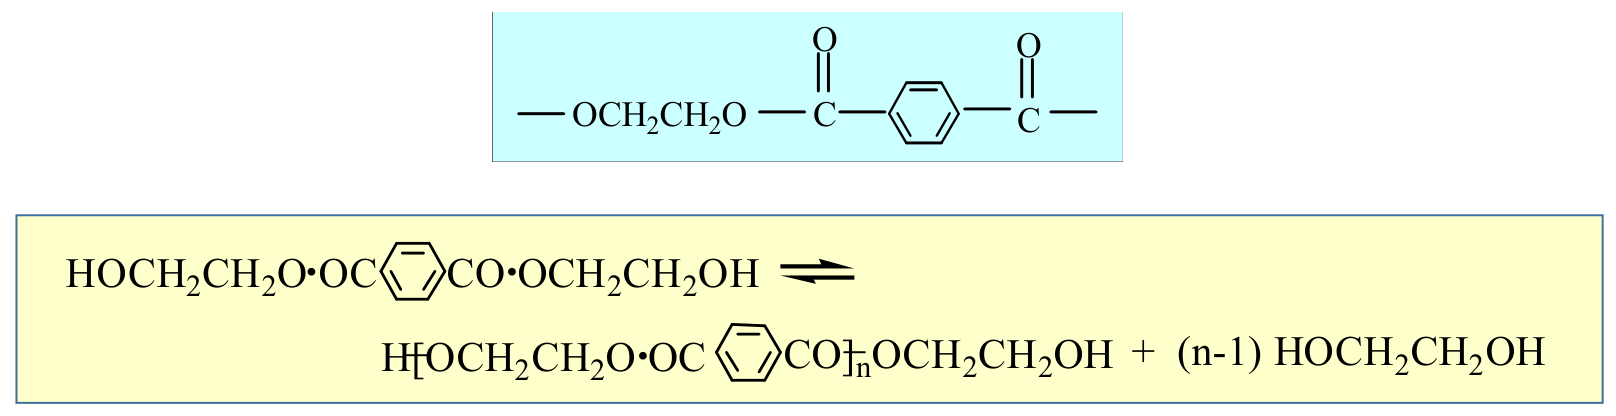
\includegraphics[width=0.96\textwidth]{figures/ch2_formula_only/pet_formula.png}
\caption{PET公式图（来源：第二章PDF第58页）}
\end{figure}

\subsubsection{聚碳酸酯（PC）}
\paragraph{定义与性能}
\begin{itemize}
  \item 工业化的聚碳酸酯主要限于双酚A型PC，属于非结晶工程塑料。
  \item 其特点是在较宽温度范围内具有良好的力学性能，同时兼具高透明性、尺寸稳定性和电绝缘性。
\end{itemize}

\paragraph{合成路线}
\begin{itemize}
  \item 酯交换法以双酚A和碳酸二苯酯为原料，通常使碳酸二苯酯过量，分阶段进行酯交换，排出苯酚并得到高分子量PC。
  \item 光气直接法则将双酚A钠盐水溶液与光气有机溶液进行界面缩聚；由于界面缩聚近似不可逆，对原料等当量比要求不如线性缩聚那样严格，工业上常加入少量单官能酚进行封端以控制分子量。
\end{itemize}
双酚A型PC的重复结构单元与反应式可表示为：
\[
\left[-\mathrm{O{-}Ar{-}C(CH_3)_2{-}Ar{-}O{-}CO-}\right]_n
\]
\[
\begin{aligned}
n\,\mathrm{HO{-}Ar{-}C(CH_3)_2{-}Ar{-}OH}+n\,\mathrm{(PhO)_2CO}
&\rightarrow
\left[-\mathrm{O{-}Ar{-}C(CH_3)_2{-}Ar{-}O{-}CO-}\right]_n \\
&\quad +2n\,\mathrm{PhOH}
\end{aligned}
\]
\begin{figure}[!htbp]
\centering
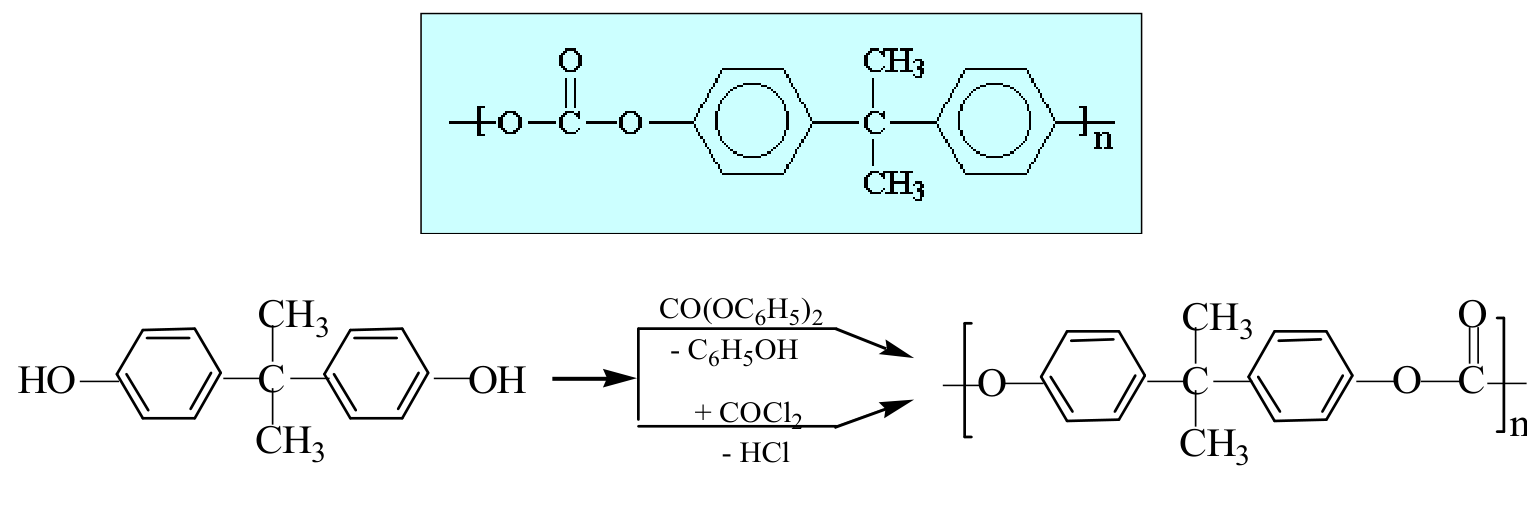
\includegraphics[width=0.96\textwidth]{figures/ch2_formula_only/pc_formula.png}
\caption{PC公式图（来源：第二章PDF第59页）}
\end{figure}

\subsubsection{聚酰胺（PA）}
\paragraph{分类与代表}
\begin{itemize}
  \item 主链含酰胺基（$-\mathrm{NHCO}-$），分脂族与芳族。
  \item 脂族聚酰胺又可分为2-2系列和2系列，前者典型代表为尼龙-66，后者典型代表为尼龙-6。
  \item 芳族聚酰胺代表包括半芳的尼龙-6T和全芳的对位芳纶PPTA；2系列芳族聚酰胺常以聚对苯甲酰胺为代表。
\end{itemize}

\paragraph{工艺要点与性能}
\begin{itemize}
  \item 尼龙-66由己二胺与己二酸缩聚而成，工业上常采用“水中预缩聚+熔融终缩聚”两段法：先制66盐保证等基团数比，再高温减压终缩聚。
  \item 尼龙-66缩聚中氨基活性高于羟基，通常无需额外催化剂；其平衡常数较大（约$K\sim 400$），工业上可在水介质预缩聚后再终缩聚。
  \item 尼龙-66兼具较高熔点、强度和耐磨性，既可作工程塑料，也可纺丝。
  \item 尼龙-6工业上多采用己内酰胺开环聚合（速率显著高于氨基酸自缩聚）；碱催化路线常用于获得高强韧、低蠕变材料。
  \item 碱催化己内酰胺开环聚合制得的材料常用于直接浇铸大型机件，工程上常称“浇铸尼龙”。
  \item 芳族聚酰胺因主链引入苯环而耐热、刚性更高；其中对位连接通常表现出更高强度和模量。
  \item 典型耐热数据可参考：$T_m(\mathrm{PA\text{-}6T})\approx 370\,^{\circ}\mathrm{C}$，$T_m(\mathrm{PPTA})\approx 530\,^{\circ}\mathrm{C}$。
  \item 2系列脂族聚酰胺中还包括长碳链尼龙与奇数尼龙：前者柔韧性、介电性和低吸水性更突出，后者常因氢键密度差异表现出较高熔点。
  \item 对位芳纶可由对苯二胺与对苯二甲酸（或对苯二甲酰氯）体系制备，是典型高强高模纤维材料来源。
  \item 对位芳纶属于典型溶致液晶高分子，代表性商品纤维为 Kevlar。
\end{itemize}
其中PA66与PA6常用反应式分别为：
\[
\begin{aligned}
n\,\mathrm{H_2N{-}(CH_2)_6{-}NH_2}+n\,\mathrm{HOOC{-}(CH_2)_4{-}COOH}
&\rightarrow
\left[-\mathrm{NH{-}(CH_2)_6{-}NH{-}CO{-}(CH_2)_4{-}CO-}\right]_n \\
&\quad +2n\,\mathrm{H_2O}
\end{aligned}
\]
\[
n\,\mathrm{(\varepsilon\text{-}caprolactam)}
\rightarrow
\left[-\mathrm{NH{-}(CH_2)_5{-}CO-}\right]_n
\]
\begin{figure}[!htbp]
\centering
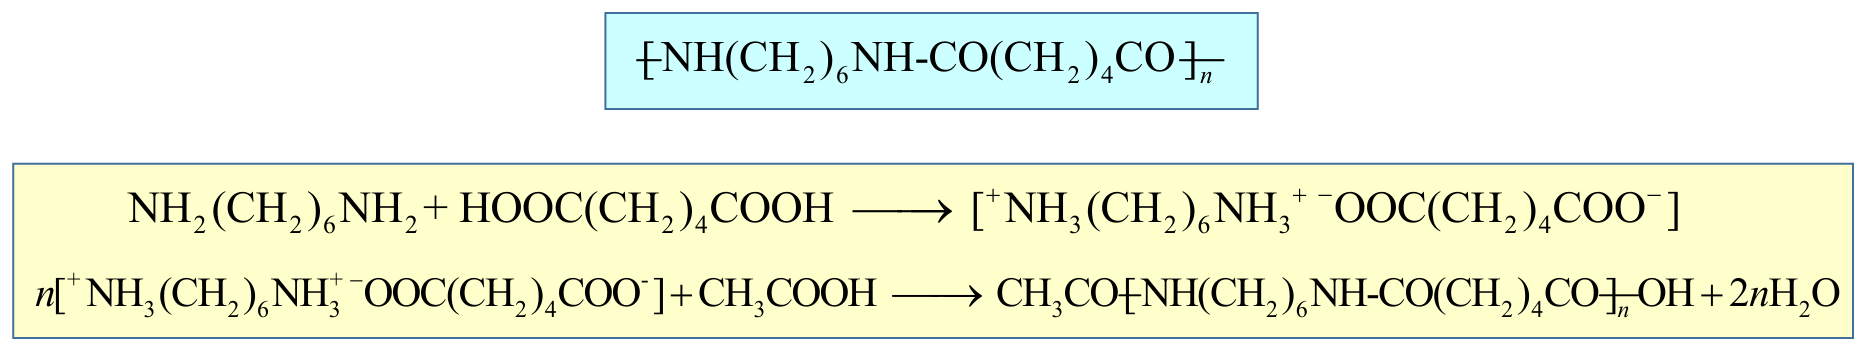
\includegraphics[width=0.96\textwidth]{figures/ch2_formula_only/pa_formula.png}
\caption{PA公式图（来源：第二章PDF第60--61页）}
\end{figure}

\subsubsection{聚酰亚胺与高性能聚合物}
\paragraph{高性能聚合物设计思路}
\begin{itemize}
  \item 高性能聚合物通常指可在$300\,^{\circ}\mathrm{C}$以上长期使用的材料。
  \item 其高温热稳定性常从三方面描述：高温下不分解（可由TGA表征）、不熔化（可由$T_m$表征）、不软化（可由热变形温度HDT表征）。
  \item 其分子设计思路主要包括：尽可能提高分子结构的规整性和对称性；在主链中引入具有较高键能并带有共振效应的芳杂环；引入可形成强氢键的基团如酰胺键、酰亚胺键；并通过提高分子堆砌紧密程度来增强热稳定性。
\end{itemize}

\paragraph{聚酰亚胺与相关材料}
\begin{itemize}
  \item 聚酰亚胺一般由芳二酐与脂二胺或芳二胺缩聚而成，常采用“两步法”：先预缩聚得可加工前驱体，再成型后终缩聚并成环固化。
  \item 当链段中的$-R-$为脂族结构时，产物往往更易溶融；$-R-$为芳环结构时，产物通常不溶不熔。
  \item 同类高性能逐步聚合物还包括聚苯并咪唑（PBI）和梯形聚合物；PBI常见原料组合可为3,3'-二氨基联苯胺与间苯二甲酸二苯酯等。
\end{itemize}
其形成过程常写为：
\[
\mathrm{H_2N{-}Ar{-}NH_2}+\mathrm{aromatic\ dianhydride}
\rightarrow\mathrm{poly(amic\ acid)}
\xrightarrow[\Delta]{\text{imidization}}
\left[-\mathrm{Ar{-}imide{-}Ar-}\right]_n+n\,\mathrm{H_2O}
\]
\begin{figure}[!htbp]
\centering
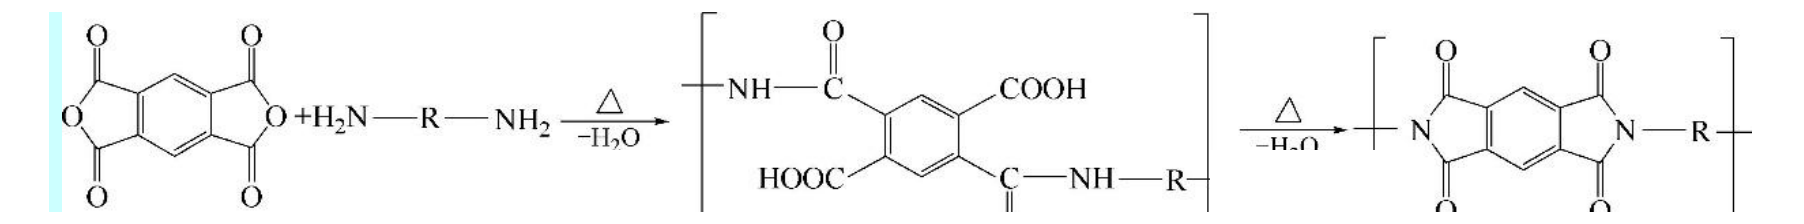
\includegraphics[width=0.96\textwidth]{figures/ch2_formula_only/pi_formula.png}
\caption{PI公式图（来源：第二章PDF第66页）}
\end{figure}

\subsubsection{聚氨酯与聚脲}
\paragraph{聚氨酯（PU）}
\begin{itemize}
  \item 聚氨酯是典型的含氮杂链聚合物，全名为聚氨基甲酸酯，可以是线性也可以是体型，属于产量很大的逐步聚合物。
  \item 理论上聚氨酯有两条合成路线：一是二氯代甲酸酯与二元胺的低温界面缩聚；二是二异氰酸酯与二元醇的聚加成。由于后一方法无副产物、二元醇更易处理，工业上主要采用二异氰酸酯与二元醇聚加成路线。
  \item 工业上常用二异氰酸酯原料包括2,4-TDI、2,6-TDI、MDI、HDI、NDI等；与聚醚/聚酯多元醇配合可覆盖弹性体、泡沫、涂料等主要产品体系。
  \item 常用多元醇原料包括聚酯二元醇与聚醚二元醇；前者耐油、耐溶剂较好，后者耐水解和低温柔性更好。
  \item 线性聚氨酯的代表是热塑性聚氨酯TPU和氨纶纤维。其分子链通常呈软段-硬段嵌段结构，硬段含芳环并可结晶、形成强氢键，相当于可逆物理交联点；软段提供柔韧性，因此材料既有弹性，又能熔融加工。
  \item 体型聚氨酯包括泡沫塑料、涂料和聚氨酯橡胶等，一般采用“预聚+交联”的两步工艺。预聚阶段多由二异氰酸酯与聚醚二醇或聚酯二醇反应，生成异氰酸酯封端预聚物；交联阶段可通过多羟基化合物、胺类扩链剂等进一步交联。
  \item 预聚物后续交联常见路径包括：异氰酸酯端基间反应、异氰酸酯与侧羟基反应、以及脲基进一步参与反应等。
  \item 聚氨酯泡沫塑料可分为软泡和硬泡：软泡多为开孔结构（缓冲、吸音），硬泡多为闭孔结构（保温）。聚氨酯涂料可分为单组分和双组分体系。
  \item 单组分聚氨酯涂料通常依赖端基与环境水分反应固化；双组分体系则在施工时混合异氰酸酯组分与含羟基树脂组分并同步交联。
  \item 聚氨酯橡胶以线性异氰酸酯封端预聚物为基础，经化学交联形成弹性体；与TPU相比，其力学性能、耐热性和耐溶剂性更好，但属于不可逆交联体系，难以重复加工。
\end{itemize}
线性PU的重复结构单元与反应式可写为：
\[
\left[-\mathrm{NH{-}COO{-}R_2{-}OCO{-}NH{-}R_1-}\right]_n
\]
\[
n\,\mathrm{OCN{-}R_1{-}NCO}+n\,\mathrm{HO{-}R_2{-}OH}
\rightarrow
\left[-\mathrm{NH{-}COO{-}R_2{-}OCO{-}NH{-}R_1-}\right]_n
\]
\begin{figure}[!htbp]
\centering
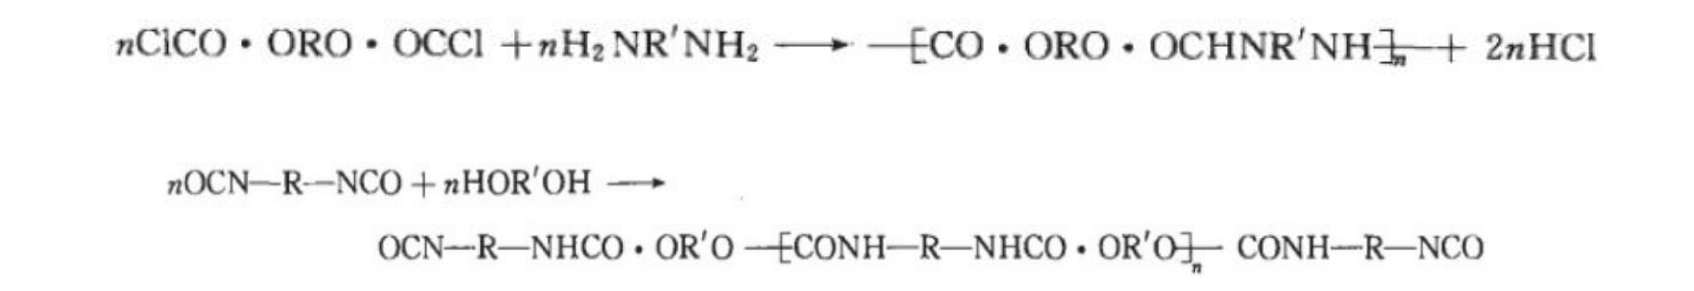
\includegraphics[width=0.96\textwidth]{figures/ch2_formula_only/pu_formula.png}
\caption{PU公式图（来源：第二章PDF第68页）}
\end{figure}

\paragraph{聚脲}
\begin{itemize}
  \item 聚脲中的脲基团极性更大、氢键更强，因此具有较高熔点、较大韧性以及较好的耐磨、耐腐蚀和耐热性能。其合成路线包括二元胺与二异氰酸酯的聚加成，以及二元胺与光气或碳酸二苯酯的界面缩聚/氨酯交换反应。
\end{itemize}
聚脲主反应可表示为：
\[
n\,\mathrm{OCN{-}R_1{-}NCO}+n\,\mathrm{H_2N{-}R_2{-}NH_2}
\rightarrow
\left[-\mathrm{NH{-}CO{-}NH{-}R_2{-}NH{-}CO{-}NH{-}R_1-}\right]_n
\]
\begin{figure}[!htbp]
\centering
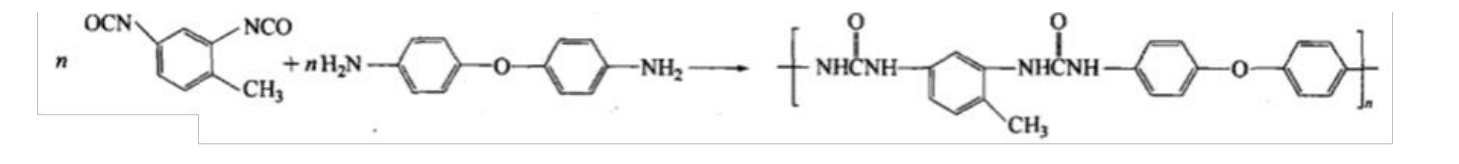
\includegraphics[width=0.96\textwidth]{figures/ch2_formula_only/polyurea_formula.png}
\caption{聚脲公式图（来源：第二章PDF第72页）}
\end{figure}

\subsubsection{环氧树脂与聚苯醚}
\paragraph{环氧树脂（EP）}
\begin{itemize}
  \item 环氧树脂预聚物通常由环氧氯丙烷与双酚A在碱催化下缩聚得到，产物主链含半芳醚键、端基为环氧基，并带有侧羟基；预聚物的聚合度$n$通常较低，因此工业上须采用“预聚+交联”两步工艺。
  \item 双酚A型环氧预聚物的聚合度通常可在 $n=0\sim 12$ 范围，对应分子量大致约为 $340\sim 3800$。
  \item 环氧树脂的交联主要利用端环氧基和侧羟基，可选用多元胺或酸酐类交联剂。伯胺类交联剂可在室温下使环氧基开环；叔胺虽无活泼氢，但在较高温度下也可促进开环；酸酐类交联剂则通常需要更高温度，通过酯化和环氧开环等途径实现交联。
  \item 环氧树脂的主要特点是粘接力强，耐腐蚀、耐溶剂、耐热和电性能好，因此广泛用于胶粘剂、涂料和纤维增强复合材料等领域。
\end{itemize}
其预聚与固化可概括为：
\[
\mathrm{BPA + epichlorohydrin}\rightarrow\mathrm{DGEBA\ prepolymer}
\]
\[
\mathrm{epoxy\ group}+\mathrm{RNH_2}
\rightarrow\mathrm{\beta\text{-}hydroxy\ amine\ linkage}
\]
\begin{figure}[!htbp]
\centering
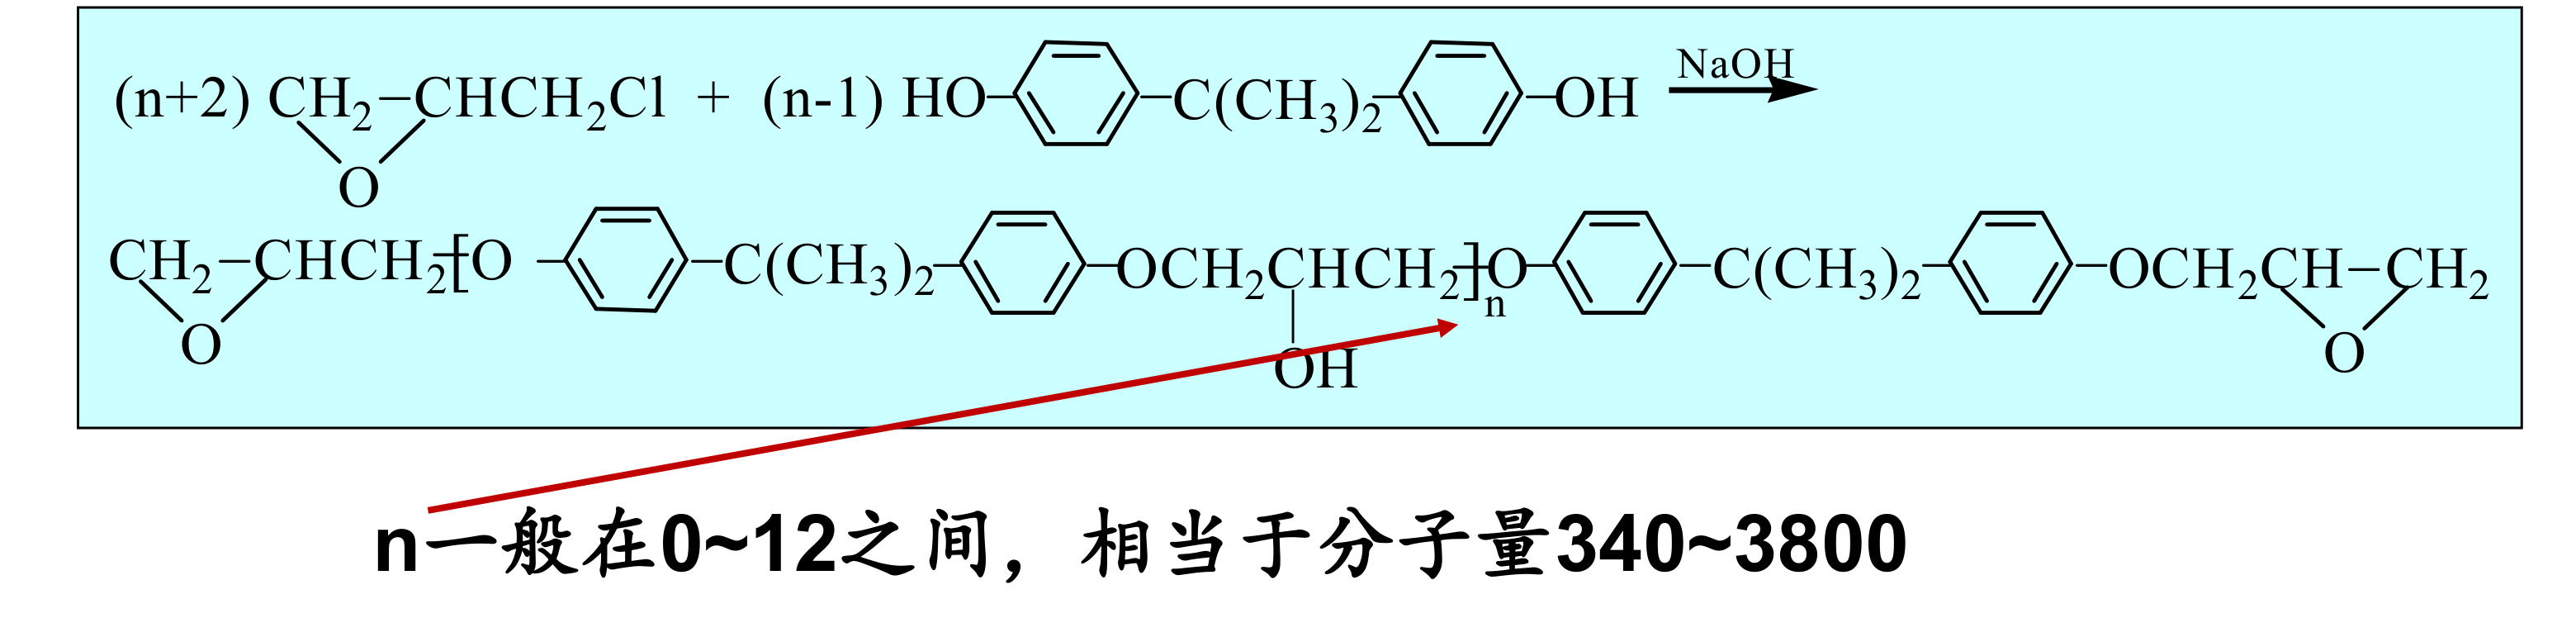
\includegraphics[width=0.96\textwidth]{figures/ch2_formula_only/epoxy_formula.png}
\caption{环氧树脂公式图（来源：第二章PDF第73页）}
\end{figure}

\paragraph{聚苯醚（PPO）}
\begin{itemize}
  \item 环氧树脂与聚苯醚的共同点之一是主链中含有半芳或全芳醚键。
  \item 聚苯醚（PPO）是线性全芳醚聚合物，属于性能优异的工程塑料，常由2,6-二甲基苯酚经氧化耦合反应制得。
\end{itemize}
PPO可写为：
\[
n\,\mathrm{HO{-}C_6H_2(CH_3)_2}
\xrightarrow[\text{Cu/amine}]{\mathrm{O_2}}
\left[-\mathrm{O{-}C_6H_2(CH_3)_2-}\right]_n+n\,\mathrm{H_2O}
\]
\begin{figure}[!htbp]
\centering
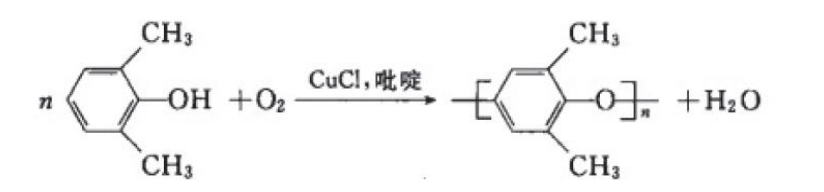
\includegraphics[width=0.96\textwidth]{figures/ch2_formula_only/ppo_formula.png}
\caption{PPO公式图（来源：第二章PDF第75页）}
\end{figure}

\subsubsection{聚砜与其他含硫杂链聚合物}
\begin{itemize}
  \item 聚砜（PSF）是主链中含砜基（$-\mathrm{SO_2}-$）的线性非晶态聚合物，分为脂族和芳族两类。脂族聚砜$T_g$较低、热稳定性差，应用有限；芳族聚砜常称聚芳醚砜或聚芳砜，具有较高$T_g$、较好的刚性和强度，属于工程塑料。
  \item 芳族聚砜通常由双酚A钠盐与4,4'-二氯二苯砜发生亲核取代反应制备。
  \item 与聚芳砜类似的高性能工程塑料还包括聚醚砜（PES）、聚醚酮（PEK）、聚醚醚酮（PEEK）等，它们的共同特点是主链中同时含有苯环、醚键和羰基等结构单元。
  \item 聚苯硫醚（PPS）属于芳族聚硫醚，具有较高耐热性和耐化学药品性。芳族PPS是结晶性工程塑料，常由对二氯苯与硫化钠经Wurtz反应合成；若引入醚键和硫醚键并存的结构，还可改善柔性和加工性能。
  \item 典型芳族PPS的热学参数常见为 $T_g\approx 85\,^{\circ}\mathrm{C}$、$T_m\approx 285\,^{\circ}\mathrm{C}$；脂族聚硫醚通常$T_g$较低、强度偏低，应用有限。
\end{itemize}
对应的形成反应可分别表示为：
\[
\begin{aligned}
n\,\mathrm{NaO{-}Ar{-}C(CH_3)_2{-}Ar{-}ONa}+n\,\mathrm{Cl{-}Ar{-}SO_2{-}Ar{-}Cl}
&\rightarrow
\left[-\mathrm{Ar{-}O{-}Ar{-}SO_2{-}Ar{-}O-}\right]_n \\
&\quad +2n\,\mathrm{NaCl}
\end{aligned}
\]
\[
n\,\mathrm{Cl{-}C_6H_4{-}Cl}+n\,\mathrm{Na_2S}
\rightarrow
\left[-\mathrm{C_6H_4{-}S-}\right]_n+2n\,\mathrm{NaCl}
\]
\begin{figure}[!htbp]
\centering
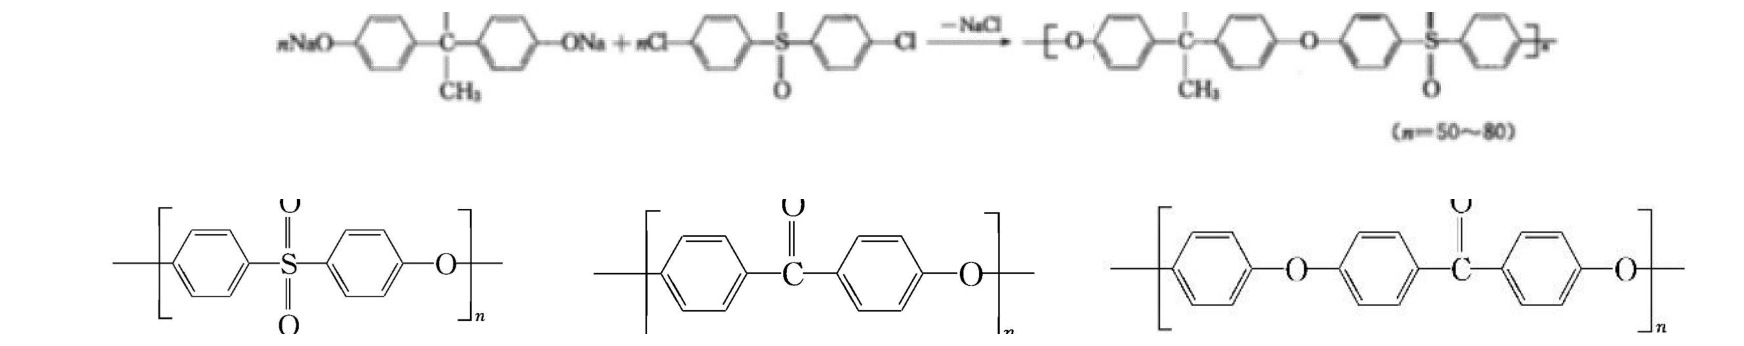
\includegraphics[width=0.96\textwidth]{figures/ch2_formula_only/psf_formula.png}
\caption{聚砜及相关高性能聚合物公式图（来源：第二章PDF第76页）}
\end{figure}

\begin{figure}[!htbp]
\centering
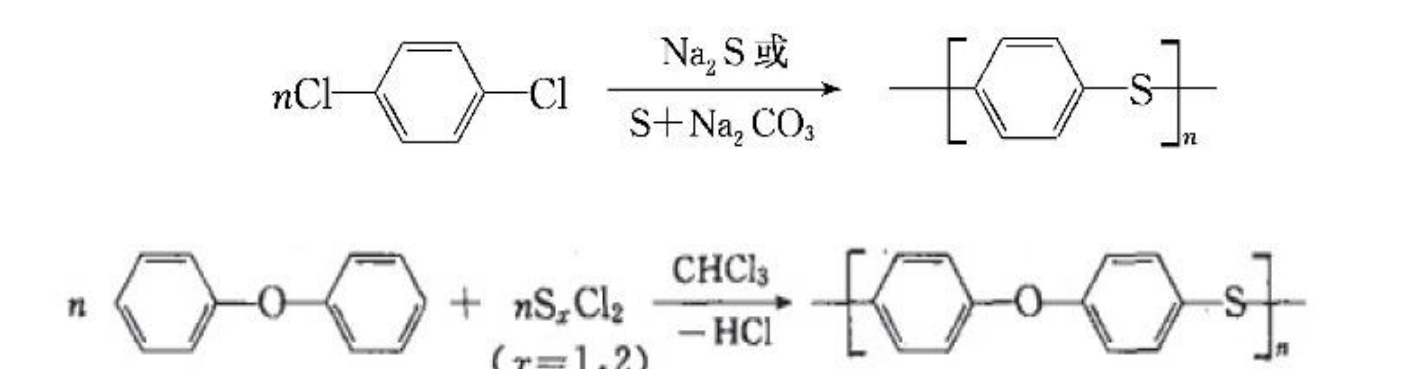
\includegraphics[width=0.96\textwidth]{figures/ch2_formula_only/pps_formula.png}
\caption{PPS公式图（来源：第二章PDF第77页）}
\end{figure}


\subsubsection{酚醛树脂（PF）}
\paragraph{组成与结构特征}
\begin{itemize}
  \item 酚醛树脂由苯酚与甲醛缩聚而成，其中苯酚可看作官能度为3、甲醛官能度为2，因此最终制品呈交联网络结构，不溶不熔。
  \item 酚醛树脂的预聚物分为无规预聚物和结构预聚物两类，分别对应碱催化和酸催化体系。
\end{itemize}

\paragraph{两类预聚体系}
\begin{itemize}
  \item 碱催化酚醛预聚物称Resoles，通常在甲醛过量条件下制备。反应先发生亲核加成形成酚醇或羟甲基酚，再进一步缩合生成多元酚醇型预聚物；此类预聚物继续加热即可交联固化，常用于胶粘剂、木工板和层压板等。
  \item 酸催化酚醛预聚物称Novolacs，通常在苯酚过量条件下制备。其机理是甲醛羰基先质子化，再在苯酚邻、对位发生亲电芳香取代，继而缩合形成由亚甲基桥随机连接的热塑性酚醛树脂。该类预聚物本身不会直接交联，需与乌洛托品（六亚甲基四胺）混合后加热，借由其分解提供亚甲基而发生交联固化。
\end{itemize}
PF网络的典型连接键与形成过程可写为：
\[
\mathrm{Ar{-}CH_2{-}Ar}\quad\text{与}\quad\mathrm{Ar{-}CH_2{-}O{-}CH_2{-}Ar}
\]
\[
\mathrm{phenol + formaldehyde}\rightarrow\mathrm{resol/novolac\ prepolymer}
\xrightarrow[\Delta]{\text{curing}}
\mathrm{crosslinked\ PF\ network}
\]
\begin{figure}[!htbp]
\centering
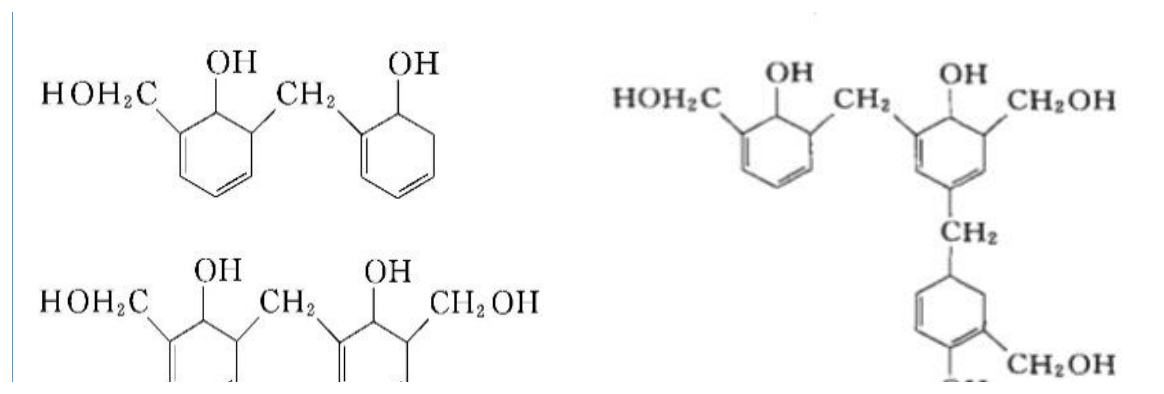
\includegraphics[width=0.96\textwidth]{figures/ch2_formula_only/pf_formula.png}
\caption{PF公式图（来源：第二章PDF第79页）}
\end{figure}

\subsubsection{氨基树脂}
\paragraph{组成与机理}
\begin{itemize}
  \item 氨基树脂由尿素或三聚氰胺与甲醛缩聚制得，主要包括脲醛树脂（UF）和密胺树脂（MF）。
  \item 脲醛树脂的预聚阶段通常在碱性条件下进行，尿素与甲醛先发生亲核加成，形成一羟甲基脲到三羟甲基脲等羟甲基衍生物；固化阶段则在中性或酸性条件下，羟基与酰胺基进一步缩合，在氮原子之间形成亚甲基桥。
\end{itemize}

\paragraph{性能与用途}
\begin{itemize}
  \item UF一般色浅或无色，硬度较高，可用作涂料、胶粘剂、层压材料和模塑品；与纤维素、固化剂、颜料等混合后可制模塑粉，也常作为木粉、碎木等材料的胶粘剂。
  \item UF模塑粉常用于低压电器和日用品部件；其胶粘体系可用于木屑板和合成板等人造板材。
  \item 密胺树脂又称三聚氰胺树脂，其合成机理与脲醛树脂相似：预聚时在微碱性条件下先形成羟甲基衍生物，固化时即使不在酸性条件下，也可仅靠加热通过羟基与氨基缩合而交联。
  \item MF的硬度和耐水性通常优于UF，常用于制作色彩鲜艳的餐具，也可用于电器制品。
\end{itemize}
UF/MF体系可用下式概括：
\[
\text{UF: }\mathrm{H_2N{-}CO{-}NH_2 + CH_2O}\rightarrow\mathrm{methylol\ urea}
\]
\[
\text{MF: }\mathrm{melamine + CH_2O}\rightarrow\mathrm{methylol\ melamine}
\xrightarrow[\Delta]{\text{acid/heat}}
\mathrm{crosslinked\ UF/MF\ network}+\mathrm{H_2O}
\]
\begin{figure}[!htbp]
\centering
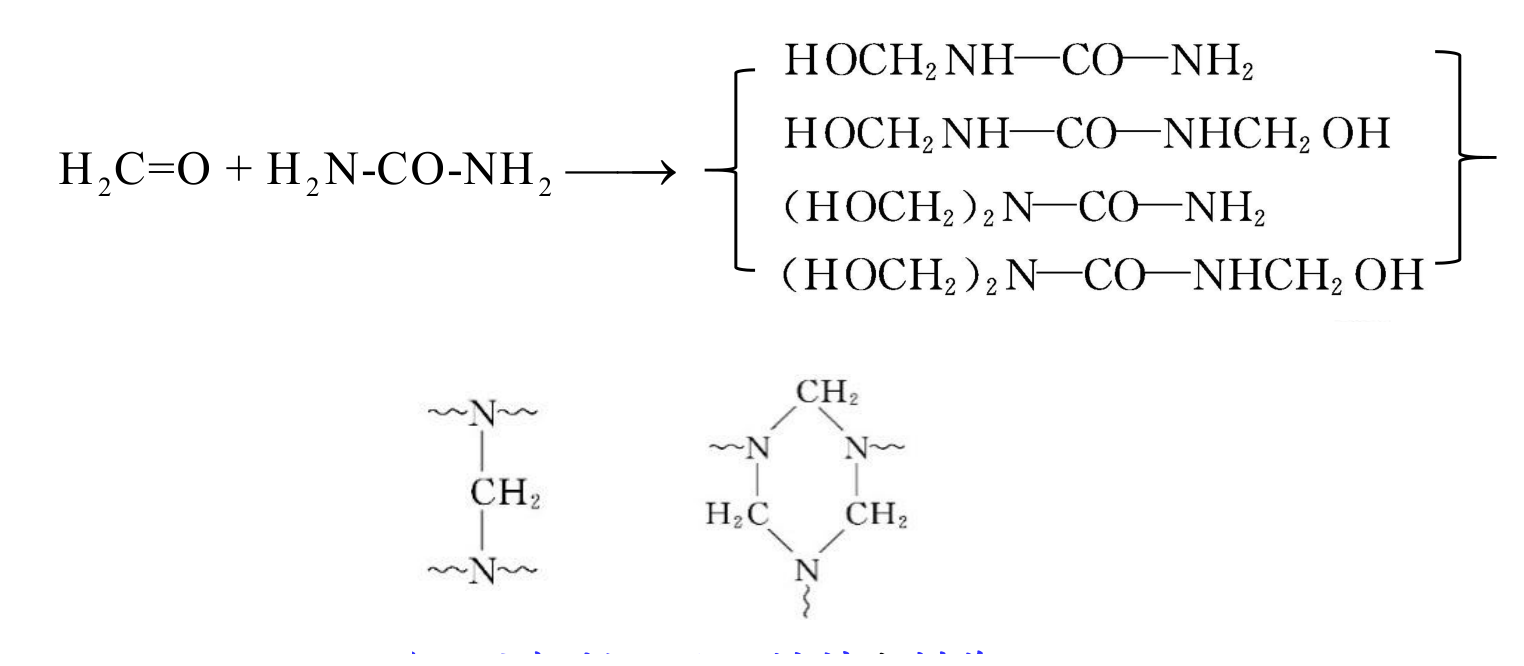
\includegraphics[width=0.96\textwidth]{figures/ch2_formula_only/uf_formula.png}
\caption{UF公式图（来源：第二章PDF第83页）}
\end{figure}

\begin{figure}[!htbp]
\centering
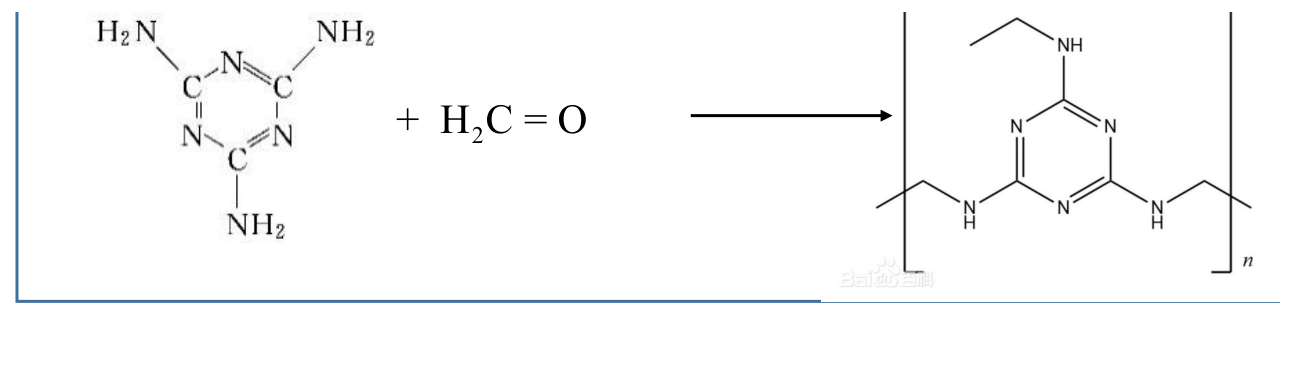
\includegraphics[width=0.96\textwidth]{figures/ch2_formula_only/mf_formula.png}
\caption{MF公式图（来源：第二章PDF第84页）}
\end{figure}



\newpage
\section{自由基聚合}
\subsection{引言}
合成高分子材料中，约70\%以上来自连锁聚合反应，例如PE、PP、PVC、PS、ABS、PTFE、PMMA、PAN、SBS、SBR、丁腈橡胶、氯丁橡胶等。

\paragraph{连锁聚合的基本条件}
\begin{itemize}
  \item 外因：体系中需要存在活性种（自由基、阳离子或阴离子）。
  \item 内因：单体分子中存在可被活性种进攻的弱键（通常为$\mathrm{C=C}$）。
\end{itemize}

\paragraph{活性种的形成}
活性种来源于共价键断裂，可分为：
\begin{itemize}
  \item 均裂：一对电子平均分给两端，形成两个自由基。
  \item 异裂：一对电子全部归属一端，形成离子对（阳离子和阴离子）。
\end{itemize}

\paragraph{连锁聚合机理特征}
连锁聚合由链引发、链增长、链终止和链转移等基元反应串并联构成：
\begin{itemize}
  \item 链引发：活性种进入链端并形成首个结构单元。
  \item 链增长：活性链连续加成单体，重复单元数增加。
  \item 链终止：活性链失活，不再增长。
  \item 链转移：活性链把活性转移给别的分子，自身失活。
\end{itemize}

\subsection{烯类单体对聚合机理的选择性}
\subsubsection{电子效应主导机理选择}
乙烯基单体$\mathrm{CH_2=CHY}$中，取代基$Y$的诱导效应与共轭效应决定活性种进攻方式。
\begin{itemize}
  \item 供电子取代基（如烷基、苯基、乙烯基）提高双键电子云密度，并稳定增长碳正离子，倾向阳离子聚合。
  \item 吸电子取代基（如$-\mathrm{CN}$、$-\mathrm{COOR}$、$-\mathrm{COR}$）降低双键电子云密度，并稳定增长碳负离子，倾向阴离子聚合。
  \item 含$\pi$-$\pi$共轭结构（如苯乙烯、丁二烯、异戊二烯）常可按三种机理聚合。
\end{itemize}

\subsubsection{典型单体说明}
\begin{itemize}
  \item 乙烯：结构对称，诱导/共轭效应弱，通常需高温高压自由基聚合。
  \item 烷基乙烯基醚：诱导效应吸电子，但$\mathrm{p}$-$\pi$共轭更强，整体偏阳离子聚合。
  \item 氯乙烯：诱导和共轭效应都较弱，主要进行自由基聚合。
\end{itemize}

\subsubsection{位阻效应先判断能否聚合}
位阻虽不决定活性种类型，但显著影响能否发生聚合：
\begin{itemize}
  \item $1,1$-二取代烯一般比单取代更易极化，较易聚合；但若两取代基都很大（如$1,1$-二苯基乙烯），常仅得到低聚物。
  \item $1,2$-二取代单体一般难均聚。
  \item 三、四取代烯烃通常难聚合（氟代体系除外）。
\end{itemize}

\paragraph{判断流程（复习重点）}
\begin{enumerate}[1)]
  \item 先看位阻，判断单体能否聚合；
  \item 再看电子效应，判断更可能属于哪类聚合机理。
\end{enumerate}

\subsection{自由基聚合机理}
\subsubsection{自由基的活性}
自由基活性与结构密切相关。过于活泼的$\mathrm{H\cdot}$、$\mathrm{CH_3\cdot}$易与双键以外部位或杂质反应；过于稳定的共轭自由基又难以引发聚合，因此真正适合引发聚合的自由基应当“活性适中”。
\begin{itemize}
  \item 初级自由基必须先形成，再与单体加成成为单体自由基；
  \item 受共轭效应和位阻效应显著稳定的自由基，多表现为稳定自由基或阻聚剂；
  \item 引发能力的本质是：既能形成自由基，又能较快加成到$\mathrm{C=C}$上。
\end{itemize}

\subsubsection{链引发}
链引发一般包括两步：
\begin{enumerate}[1)]
  \item 引发剂分解：
  \[
  \mathrm{I \xrightarrow{k_d} 2R\cdot}
  \]
  \item 初级自由基加成单体：
  \[
  \mathrm{R\cdot + M \xrightarrow{k_i} RM\cdot}
  \]
\end{enumerate}
\[
R_d=k_d[I],\qquad R_i=2fk_d[I]
\]
特点：分解常为吸热过程，$E_d\approx105\sim150\,\mathrm{kJ\cdot mol^{-1}}$，$k_d$常在$10^{-4}\sim10^{-6}\,\mathrm{s^{-1}}$量级；引发通常是整个连锁过程最慢的步骤。

\subsubsection{链增长}
\[
\mathrm{RM_n\cdot + M \xrightarrow{k_p} RM_{n+1}\cdot}
\]
特点：放热、活化能低、速率快。常采用等活性假定：
\[
k_{p1}=k_{p2}=\cdots=k_p
\]
链增长常为放热过程，聚合热约$55\sim95\,\mathrm{kJ\cdot mol^{-1}}$，活化能常在$20\sim34\,\mathrm{kJ\cdot mol^{-1}}$。连接方式可有头-尾、头-头，其中头-尾连接通常占主导。

\subsubsection{链终止}
自由基活性高，终止通常为双基终止：
\begin{itemize}
  \item 偶合终止：两链自由基直接结合成共价键。
  \item 歧化终止：一条链夺取另一条链原子（常为氢），形成一饱和一不饱和链端。
\end{itemize}
终止活化能低，常在$8\sim21\,\mathrm{kJ\cdot mol^{-1}}$，反应很快，且易受扩散控制。常见经验结论：
\begin{itemize}
  \item 苯乙烯聚合多以偶合终止为主；
  \item MMA在$60^\circ\mathrm{C}$以上常以歧化终止为主，低于该温度两种方式可并存。
\end{itemize}

\subsubsection{链转移}
\[
\mathrm{RM\cdot + YS \xrightarrow{k_{tr}} RMH + S\cdot}
\]
链转移可发生在单体、引发剂、溶剂和大分子上。原活性链失活后，新的自由基可能继续引发；因此链转移会降低分子量，并可能引入支化（如LDPE中向大分子转移）。

\subsubsection{机理特征小结}
\begin{itemize}
  \item 微观上是慢引发、快增长、速终止；
  \item 链引发最慢，因此引发速率往往是控制聚合速率的关键；
  \item 只有链增长使聚合度增加；
  \item 反应混合物的主体通常是单体和聚合物，中间自由基浓度极低；
  \item 延长聚合时间主要提高转化率，对分子量影响相对较小。
\end{itemize}

\subsection{引发剂}
\subsubsection{引发剂与催化剂区别}
引发剂在反应中被消耗并进入链端；催化剂本身不被消耗，反应后仍可回收。

\subsubsection{常见引发剂类型}
\begin{itemize}
  \item 偶氮类：如AIBN（低活性）、ABVN（中活性），分解放出$\mathrm{N_2}$，便于测定分解速率。
  \item 有机过氧类：过氧化二烷基、过氧化二酰基多为低活性（如DCP、BPO）；过氧酯多为中活性（如BPP）；过氧化二碳酸酯多为高活性。
  \item 无机过氧类：如过硫酸钾、过硫酸铵，水溶性好，适于乳液/水溶液聚合。
\end{itemize}

\subsubsection{氧化-还原引发体系}
由氧化剂与还原剂构成，自由基来源于电子转移，活化能低，可低温引发。
\begin{itemize}
  \item 水溶性体系：过氧化氢/亚铁盐、过硫酸盐/亚硫酸盐等。
  \item 油溶性体系：有机过氧化物/叔胺等。
\end{itemize}

\subsubsection{分解动力学与活性表征}
\[
\mathrm{I \xrightarrow{k_d} 2R\cdot},\qquad -\frac{d[I]}{dt}=k_d[I]
\]
积分后：
\[
\ln\frac{[I]}{[I]_0}=-k_dt,\qquad [I]=[I]_0e^{-k_dt}
\]
半衰期：
\[
t_{1/2}=\frac{\ln2}{k_d}
\]
\[
k_d=A_d\exp\!\left(-\frac{E_d}{RT}\right)
\]
通常$k_d$越大或$t_{1/2}$越短，引发剂活性越高。工业上常用$60^\circ\mathrm{C}$下的半衰期粗分：$t_{1/2}<1\,\mathrm{h}$为高活性，$1\sim6\,\mathrm{h}$为中活性，$>6\,\mathrm{h}$为低活性。

\subsubsection{引发剂效率}
引发效率$f$一般在$0.5\sim0.8$，受诱导分解与笼蔽效应影响。
\begin{itemize}
  \item 诱导分解：初级自由基先与引发剂反应，降低有效引发比例。
  \item 笼蔽效应：初级自由基在“笼子”中复合或副反应，未及时逃逸至单体双键。
  \item AIBN几乎无诱导分解，而ROOH等氢过氧化物更易发生诱导分解。
  \item 引发剂浓度越高，越易诱导分解；活性较高的单体（如AN、St）通常更易获得较高$f$值。
\end{itemize}

\subsubsection{引发剂选择原则}
\begin{itemize}
  \item 与聚合温度匹配：通常选$t_{1/2}$与聚合时间同数量级的引发剂。
  \item 与聚合方法匹配：本体/悬浮/有机溶液常用油溶性引发剂，乳液/水溶液常用水溶性体系。
  \item 选择初级自由基能与单体快速接触的引发剂。
  \item 工业间歇聚合常采用高-低（或高-中）活性引发剂复配，或先常温聚合再升温后聚合，以尽量使聚合过程匀速并减少残余引发剂。
  \item 低活性引发剂用量常偏大，高活性用量偏小，典型范围约为单体质量的$0.01\%\sim0.1\%$。
  \item 兼顾安全、颜色、毒性、储运与成本。
\end{itemize}

\subsection{其他引发作用}
\subsubsection{热引发}
不加引发剂，靠热使单体形成自由基而聚合。实际意义在于说明单体存在自聚风险，储存与运输需加阻聚措施。

\subsubsection{光引发}
光引发包括光直接引发、光引发剂引发和光敏剂间接引发。
\[
E=\frac{N_Ahc}{\lambda}
\]
\begin{itemize}
  \item 当$\lambda=300\,\mathrm{nm}$时，$1\,\mathrm{mol}$光子的能量约$400\,\mathrm{kJ\cdot mol^{-1}}$，足以超过多数化学反应活化能；
  \item 选择性强，可通过开关光源实现速率可控；
  \item 总活化能低，适于低温操作，副反应少；
  \item 典型应用：光固化油墨、光刻胶、印刷制版等。
\end{itemize}

\subsubsection{辐射引发}
\begin{itemize}
  \item 高能辐射线可使分子形成离子自由基，能量远高于普通光引发；
  \item 选择性较差，可在多种化学键上断裂并生成多种初级自由基；
  \item 穿透力强，可用于固相聚合。
\end{itemize}

\subsubsection{等离子体与微波引发}
\begin{itemize}
  \item 等离子体引发可在气相引发、液相或固相表面增长，常用于酶固定化、表面接枝和成膜。
  \item 等离子体态聚合可使许多有机物解离、重排并再结合，常形成交联膜层，常见于CVD类表面沉积。
  \item 高分子等离子体表面处理可实现刻蚀、粗面化、引入极性基团或表面氟化，从而改善粘接、亲水或防水防油性能。
  \item 微波引发兼具热效应与非热效应；无引发剂时可促进热引发，有引发剂时可加速聚合并降低引发剂用量或聚合温度。
\end{itemize}

\subsection{聚合速率}
\subsubsection{基本定义与宏观阶段}
聚合速率：
\[
R_p=-\frac{d[M]}{dt}=\frac{d[P]}{dt}
\]
转化率：
\[
C=\frac{[M]_0-[M]}{[M]_0}\times100\%
\]
典型$C$-$t$曲线呈$S$形，可分诱导期、初期（近匀速）、中期（自动加速）、后期（减速）。

\subsubsection{微观聚合动力学的研究方法}
\begin{itemize}
  \item 直接法：测未反应单体量，如溴量法测双键变化；或定期取样沉淀、干燥并称量聚合物。
  \item 间接法：利用比容、黏度、光谱等物理量变化反推聚合进程。
  \item 膨胀计法的核心依据是：聚合物密度通常高于单体，聚合过程中体系体积收缩，且体积变化与转化率近似呈线性关系。
\end{itemize}

\subsubsection{低转化率下微观动力学（自由基聚合普遍式）}
采用长链假定、等活性假定和稳态假定：
\[
R_i=2fk_d[I],\qquad R_t=2k_t[M\cdot]^2,\qquad R_i=R_t
\]
得到：
\[
[M\cdot]=\left(\frac{fk_d[I]}{k_t}\right)^{1/2}
\]
\[
R_p=k_p[M][M\cdot]=k_p\left(\frac{fk_d}{k_t}\right)^{1/2}[I]^{1/2}[M]
\]
即：
\[
R_p\propto [I]^{1/2}[M]
\]

\subsubsection{基元反应速率常数与速率范围}
\begin{itemize}
  \item 链引发：$k_d\sim10^{-4}\sim10^{-6}\,\mathrm{s^{-1}}$，$f\approx0.6\sim0.8$，$[I]$常为$10^{-2}\sim10^{-4}\,\mathrm{mol\cdot L^{-1}}$，故$R_i$常仅$10^{-8}\sim10^{-10}\,\mathrm{mol\cdot L^{-1}\cdot s^{-1}}$。
  \item 链增长：$k_p\sim10^2\sim10^4\,\mathrm{L\cdot mol^{-1}\cdot s^{-1}}$，$[M]$常为$1\sim10\,\mathrm{mol\cdot L^{-1}}$，故$R_p$约$10^{-4}\sim10^{-6}\,\mathrm{mol\cdot L^{-1}\cdot s^{-1}}$。
  \item 链终止：$k_t\sim10^6\sim10^8\,\mathrm{L\cdot mol^{-1}\cdot s^{-1}}$，但$[M\cdot]$仅$10^{-7}\sim10^{-9}\,\mathrm{mol\cdot L^{-1}}$，故$R_t$与$R_i$同量级。
\end{itemize}

\subsubsection{温度影响}
当引发剂引发时，总活化能近似为：
\[
E=E_p-\frac{1}{2}E_t+\frac{1}{2}E_d
\]
通常$E>0$，故温度升高，$R_p$增大；但聚合度一般随温度升高而下降（见后文）。

\subsubsection{凝胶效应与自动加速}
中期体系黏度升高，$k_t$因扩散受限显著下降，而$k_p$下降较小，导致$k_p/k_t^{1/2}$上升，出现自动加速（Trommsdorff效应）。
\begin{itemize}
  \item 自动加速的起点并不一定等于凝胶效应的起点；扩散控制可能更早出现，但未必足以抵消$[M]$和$[I]$的降低。
  \item 对均相聚合体系，明显自动加速通常只在双基终止体系中更突出；单基终止体系虽也可有扩散控制，但自动加速常不明显。
  \item 非均相沉淀聚合若增长与终止所受扩散限制差异很大，也可能出现明显自动加速。
  \item 后果：放热积累，可能引发爆聚风险。
  \item 工艺对策：强化传热、降低体系黏度、采用悬浮/乳液/溶液等分散式聚合方式。
\end{itemize}

\subsection{动力学链长和聚合度}
\subsubsection{动力学链长}
定义：一个活性种从引发到真正失活所消耗的单体分子数，记作$\nu$。
\[
\nu=\frac{R_p}{R_t}
\]
低转化率下：
\[
\nu\propto \frac{[M]}{[I]^{1/2}}
\]

\subsubsection{与聚合度关系}
\begin{itemize}
  \item 歧化终止：$\bar{X}_n=\nu$
  \item 偶合终止：$\bar{X}_n=2\nu$
  \item 混合终止：$\bar{X}_n=(C+2D)\nu$（$C,D$分别为歧化与偶合分率）
\end{itemize}

\subsubsection{温度对聚合度影响}
链转移与终止过程综合作用下，聚合温度升高通常使$\bar{X}_n$降低，这也是工业上用温度调控分子量的重要依据。

\subsection{链转移反应和聚合度}
\subsubsection{链转移对象}
活性链可向单体、引发剂、溶剂及大分子转移：
\begin{itemize}
  \item 向单体：决定部分体系（如VC）聚合度上限；
  \item 向引发剂：降低引发效率并降低聚合度；
  \item 向溶剂：溶液聚合中常使分子量下降；
  \item 向大分子：导致支化或交联。
\end{itemize}
\[
R_{tr,M}=k_{tr,M}[RM\cdot][M],\quad
R_{tr,I}=k_{tr,I}[RM\cdot][I],\quad
R_{tr,S}=k_{tr,S}[RM\cdot][S]
\]

\subsubsection{Mayo方程（复习核心公式）}
\[
\frac{1}{\bar{X}_n}=\frac{1}{\bar{X}_{n,0}}+C_M\frac{[M]}{[M]}+C_I\frac{[I]}{[M]}+C_S\frac{[S]}{[M]}
\]
常写为近似形式：
\[
\frac{1}{\bar{X}_n}=\frac{1}{\bar{X}_{n,0}}+C_M+C_I\frac{[I]}{[M]}+C_S\frac{[S]}{[M]}
\]
其中$C_j=k_{tr,j}/k_p$为链转移常数。

\subsubsection{典型结论}
\begin{itemize}
  \item 常见单体$C_M$较小，常在$10^{-5}$量级；
  \item VC向单体链转移较强，因此PVC工业上常通过温度来调控聚合度；
  \item 在本体聚合中，可通过$\left(\frac{2R_p}{k_p[M]^2}\right)\frac{1}{\bar{X}_n}$对$[I]/[M]$作图求$C_I$；在溶液聚合中，可通过$1/\bar{X}_n$对$[S]/[M]$作图求$C_S$；
  \item 硫醇类$C_S$较大，常作分子量调节剂（链转移剂）；
  \item 向大分子转移会引入长支链或短支链（LDPE的重要结构来源）。
\end{itemize}

\subsection{聚合度分布}
\subsubsection{歧化终止时}
用概率法可得分布函数，结果要点：
\begin{itemize}
  \item 数均聚合度：$\bar{X}_n\approx\dfrac{1}{1-p}$
  \item 重均聚合度：$\bar{X}_w\approx\dfrac{1+p}{1-p}$
  \item 分布指数：$\dfrac{\bar{X}_w}{\bar{X}_n}\approx2$
\end{itemize}

\subsubsection{偶合终止时}
\begin{itemize}
  \item 数均聚合度约为歧化终止的2倍；
  \item 分布指数理论值约$1.5$。
\end{itemize}

\paragraph{小结}
同等条件下，偶合终止更有利于提高聚合度并缩窄分布；实际体系常为两种终止方式并存。

\subsection{阻聚作用和阻聚剂}
\subsubsection{基本概念}
\begin{itemize}
  \item 阻聚剂：使聚合反应完全停止或在一段时间内停止。
  \item 缓聚剂：仅降低聚合速率，不使反应完全停止。
\end{itemize}
阻聚会引入诱导期$t_i$：
\[
R_i=\frac{n[Z]_0}{t_i}
\]
其中$[Z]_0$为阻聚剂初始浓度，$n$为单位阻聚剂可捕捉的自由基数。

\subsubsection{常见阻聚剂类型}
\begin{itemize}
  \item 稳定自由基型：如DPPH、TEMPOL等；
  \item 变价金属盐型：通过电子转移使自由基失活；
  \item 加成型：如氧、苯醌衍生物、硝基化合物；
  \item 链转移型：酚类、芳胺类等，通过夺氢形成低活性自由基。
\end{itemize}

\subsubsection{自阻聚现象}
烯丙基单体常表现出明显自阻聚：链转移倾向大于链增长（$k_{tr}\gg k_p$），故聚合速率低、产物分子量低。

\subsubsection{阻聚效率与诱导期利用}
\begin{itemize}
  \item 阻聚效率常用阻聚常数$C_z=k_z/k_p$衡量，$C_z$越大，说明阻聚剂越容易与自由基竞争。
  \item 高效阻聚剂在诱导期内的消耗常近似与其浓度无关，可近似视为零级过程。
  \item DPPH、$\mathrm{FeCl_3}$等可快速按近似$1{:}1$捕捉自由基，常用于比色法测定引发速率。
\end{itemize}

\subsection{自由基寿命和链增长、链终止速率常数的测定}
自由基寿命定义为稳态下活性自由基从生成到消失的平均存活时间：
\[
\tau=\frac{[M\cdot]_s}{R_t}=\frac{1}{2k_t[M\cdot]_s}
\]
由
\[
R_p=k_p[M][M\cdot]_s
\]
可联立求$k_p$与$k_t$。实验上常结合光闸法、ESR等方法获取$\tau$或$[M\cdot]_s$后反推相关速率常数。

\subsection{“活性”自由基聚合}
\subsubsection{目标与思想}
传统自由基聚合因不可逆终止导致分子量分布宽、结构可控性差。所谓“活性”自由基聚合的核心是：通过可逆失活/再活化平衡，将大部分链保持在休眠态，显著降低自由基瞬时浓度，实现可控聚合。

\subsubsection{三类代表方法}
\begin{itemize}
  \item NMP：氮氧稳定自由基调聚法，机理直观，最早实现“活性”自由基聚合；但单体适用范围较窄，常需较高温。
  \item ATRP：原子转移可逆失活，适用于多数苯乙烯类、丙烯酸酯和甲基丙烯酸酯单体，但需金属络合催化体系并处理金属残留。
  \item RAFT：可逆加成-裂解-链转移法，条件最接近传统自由基聚合，适用单体范围最广，但RAFT试剂常有颜色、气味且对光热较敏感。
\end{itemize}

\subsubsection{共同特征}
\begin{itemize}
  \item 分子量随转化率近线性增加；
  \item 可合成嵌段、接枝、星形等结构；
  \item 分布可显著变窄（常见$\bar{X}_w/\bar{X}_n\approx1.1\sim1.3$），但并非绝对“无终止”。
\end{itemize}

\subsubsection{动力学提示}
\begin{itemize}
  \item NMP/ATRP中，活性链与休眠链之间可逆终止控制自由基浓度；
  \item RAFT中主要为可逆链转移，常见一定缓聚现象与中间态自由基稳定化有关。
\end{itemize}

\subsubsection{动力学与局限补充}
\begin{itemize}
  \item NMP和ATRP通过可逆失活使活性自由基浓度维持在极低水平，因此聚合速率通常慢于传统自由基聚合。
  \item RAFT原则上不改变传统自由基聚合速率方程的基本形式，但中间态自由基可能引起缓聚。
  \item “活性”自由基聚合并非真正零终止体系，仍可能存在约$10\%$左右死聚物，因此只是接近活性聚合。
  \item 若希望$\bar{X}_w/\bar{X}_n$进一步接近1，通常需要足够多的激活/失活循环。
\end{itemize}

\subsection{聚合方法及重要的自由基聚合产物}
\subsubsection{概述}
工业自由基聚合主要包括：本体聚合、溶液聚合、沉淀/分散聚合、悬浮聚合和乳液聚合。实际选择时，要在产品性能、过程安全、传热控温和成本之间折中。

\subsubsection{本体聚合}
本体聚合是不加其他介质、只有单体本身在引发剂、热或光作用下进行的聚合。基本组分通常只有单体和能溶于单体的引发剂，聚合场所就在本体内。
\begin{itemize}
  \item 优点：产品纯净、设备相对简单、可连续化。
  \item 缺点：体系黏度高、传热困难、易出现凝胶效应、自动加速与爆聚。
  \item 苯乙烯连续本体（共）聚合是GPPS、SAN、R-SMA、HIPS、ABS的重要工业路线，常采用多釜串联、逐步升温并辅以脱挥。
  \item MMA间歇本体聚合制PMMA时，常先预聚到一定黏度后再转入模板中缓慢聚合，最后升温后聚合以减少残余单体。
  \item 乙烯高压本体聚合制LDPE需在高温高压下进行，链转移到大分子显著，故产物支链多、密度低、结晶度较低。
\end{itemize}

\subsubsection{溶液聚合}
真正的溶液聚合属于均相聚合：单体、引发剂、溶剂与生成的聚合物都溶于同一相中。
\begin{itemize}
  \item 优点：易撤热控温，可减弱自动加速。
  \item 缺点：聚合速率偏慢，溶剂回收能耗高，易发生向溶剂链转移。
  \item 多用于聚合物溶液可直接使用的场合，如腈纶纺丝液、PVAc/EVA体系、涂料树脂溶液。
  \item 丙烯腈连续溶液共聚可直接制得腈纶纺丝液，故称“一步法腈纶”；VAc在甲醇中聚合得PVAc后再醇解可得PVA，继续缩醛化可得维尼纶。
  \item VAc与乙烯的溶液共聚可制EVA溶液，进一步醇解后得到EVOH阻隔材料。
\end{itemize}

\subsubsection{沉淀或分散聚合}
引发剂、单体和介质互溶，但生成的聚合物不溶于介质。与溶液聚合相比，其优点是聚合物易于分离、洗涤和纯化；颗粒相本身也可能成为重要反应场所。
\begin{itemize}
  \item 丙烯腈水相沉淀聚合是“二步法腈纶”的基础路线，常在水中连续共聚后得到淤浆，再分离、干燥并送纺丝厂重新溶解纺丝。
  \item TFE分散聚合制PTFE时，体系虽加入少量表面活性剂，但其浓度低于CMC，主要作用是防止粒子聚并，因此习惯上仍称分散聚合而非真正乳液聚合。
\end{itemize}

\subsubsection{悬浮聚合}
\begin{itemize}
  \item 组分：单体、油溶性引发剂、水、分散剂。
  \item 反应场所在单体液滴中，因此每个液滴都近似于一个微型本体聚合反应器，动力学近似本体聚合。
  \item 液滴粒径取决于搅拌剪切力、界面张力与分散剂的共同作用；搅拌越强，颗粒一般越细。
  \item 颗粒形态还受分散剂种类和浓度、水油比、聚合温度、引发剂用量与单体结构影响。
  \item 常用分散剂包括PVA、明胶、纤维素、淀粉以及滑石粉、高岭土等无机细粒。
  \item 典型产品：PVC悬浮树脂、PS珠粒和发泡聚苯乙烯（EPS）等。
\end{itemize}

\subsubsection{乳液聚合}
\begin{itemize}
  \item 组分：通常为油溶性单体、水、水溶性引发剂和乳化剂，体系多为O/W型。
  \item 反应场所：增溶胶束或乳胶粒，而不是单体液滴本身。
  \item 优点：传热控温好、聚合速率快、可得较高分子量，部分胶乳可直接使用。
  \item 缺点：制得固体产品时后处理较麻烦，乳化剂也较难彻底除尽。
\end{itemize}

\subsubsection{乳化剂与乳化作用}
\begin{itemize}
  \item 常见乳化剂分为阴离子型、阳离子型、两性型和非离子型；乳液聚合中最常用的是阴离子型，非离子型多作配合乳化剂。
  \item 阴离子乳化剂的两个高频参数是CMC和三相平衡点：经典乳液聚合要求乳化剂浓度高于CMC，聚合温度高于三相平衡点。
  \item 非离子乳化剂常用HLB值和浊点描述性能；O/W型乳液聚合常需HLB在$8\sim18$之间，且聚合温度应低于浊点。
  \item 乳化剂的本质作用是降低界面张力并稳定液滴、胶束和乳胶粒，使体系难以分层。
\end{itemize}

\subsubsection{乳液聚合机理与动力学}
经典乳液聚合中，加入浓度高于CMC的乳化剂后，体系通常包含单体液滴、增溶胶束和水相中少量溶解单体三相。成核可分两类：
\begin{itemize}
  \item 胶束成核：适用于水溶性较小的单体，如苯乙烯。
  \item 均相成核：适用于水溶性较大的单体，如醋酸乙烯酯。
\end{itemize}
按乳胶粒数和速率变化，经典乳液聚合分三阶段：
\begin{enumerate}[1)]
  \item 成核期：乳胶粒数增加，$R_p$上升；
  \item 恒速期：乳胶粒数近恒定，$R_p$近恒定；
  \item 降速期：单体液滴耗尽后，$R_p$下降。
\end{enumerate}
恒速期动力学常写作：
\[
R_p=\frac{k_p[M]N\bar{n}}{N_A}
\]
\[
\bar{X}_n\approx \frac{k_p[M]N\bar{n}}{\rho}
\]
其中$N$为单位体积中的乳胶粒数，$\bar{n}$为每个乳胶粒中的平均自由基数，$\rho$为总自由基生成速率。经典$0$-$1$态模型认为胶粒很小，只能容纳$0$个或$1$个自由基，因此常有$\bar{n}\approx0.5$。这说明：
\begin{itemize}
  \item 乳液聚合中$N$极大，因此在较高聚合速率下仍可保持较低的局部自由基终止概率；
  \item $N$通常随乳化剂用量和自由基生成速率增加而增大；
  \item 提高乳胶粒数$N$，往往可以同时提高聚合速率和聚合度，这是乳液聚合与其他方法的重要差异。
\end{itemize}

\subsubsection{乳液聚合应用与进展}
\begin{itemize}
  \item 传统应用：合成橡胶胶乳、ABS/MBS改性体系、PVC糊树脂，以及可直接使用的PVAc、丙烯酸酯类涂料和胶黏剂胶乳。
  \item 种子乳液聚合：先制备小粒径种子，再溶胀后继续聚合，可把粒径由常规的$100\sim150\,\mathrm{nm}$放大到微米级。
  \item 核壳乳液聚合：可制得软核硬壳或硬核软壳粒子，常用于ABS高接枝粉和高性能涂料。
  \item 活性乳液聚合：利用乳胶粒的“隔离效应”抑制双基终止，有利于兼顾较高速率与较高分子量，但需防止乳液失稳。
  \item 细乳液聚合：通过强剪切把单体分散成$30\sim500\,\mathrm{nm}$液滴，液滴本身就是反应场所，适于制功能性胶乳。
  \item 微乳液聚合：单体含量低、乳化剂含量高，最终粒径更小，润湿、流平和渗透性能突出。
  \item 反相乳液聚合：先形成W/O乳液后聚合，常用于丙烯酰胺等水溶性单体。
  \item 无皂乳液聚合：利用引发剂残基或极性共单体使聚合物自身带表面活性，可得到表面洁净、粒径分布窄的功能微球。
\end{itemize}

\paragraph{本章复习主线}
建议按“单体选择性$\rightarrow$基元反应$\rightarrow$速率与聚合度$\rightarrow$分布与阻聚$\rightarrow$可控自由基聚合$\rightarrow$工业方法”六步回顾。

\end{document}

